% Format teze zasnovan je na paketu memoir
% http://tug.ctan.org/macros/latex/contrib/memoir/memman.pdf ili
% http://texdoc.net/texmf-dist/doc/latex/memoir/memman.pdf
% 
% Prilikom zadavanja klase memoir, navedenim opcijama se podešava 
% veličina slova (12pt) i jednostrano štampanje (oneside).
% Ove parametre možete menjati samo ako pravite nezvanične verzije
% mastera za privatnu upotrebu (na primer, u b5 varijanti ima smisla 
% smanjiti 
\documentclass[12pt,oneside]{memoir} 

% Paket koji definiše sve specifičnosti master rada Matematičkog fakulteta
\usepackage[latinica]{matfmaster} 
%
% Podrazumevano pismo je ćirilica.
%   Ako koristite pdflatex, a ne xetex, sav latinički tekst na srpskom jeziku
%   treba biti okružen sa \lat{...} ili \begin{latinica}...\end{latinica}.
%
% Opicija [latinica]:
%   ako želite da pišete latiniciom, dodajte opciju "latinica" tj.
%   prethodni paket uključite pomoću: \usepackage[latinica]{matfmaster}.
%   Ako koristite pdflatex, a ne xetex, sav ćirilički tekst treba biti
%   okružen sa \cir{...} ili \begin{cirilica}...\end{cirilica}.
%
% Opcija [biblatex]:
%   ako želite da koristite reference na više jezika i umesto paketa
%   bibtex da koristite BibLaTeX/Biber, dodajte opciju "biblatex" tj.
%   prethodni paket uključite pomoću: \usepackage[biblatex]{matfmaster}
%
% Opcija [b5paper]:
%   ako želite da napravite verziju teze u manjem (b5) formatu, navedite
%   opciju "b5paper", tj. prethodni paket uključite pomoću: 
%   \usepackage[b5paper]{matfmaster}. Tada ima smisla razmisliti o promeni
%   veličine slova (izmenom opcije 12pt na 11pt u \documentclass{memoir}).
%
% Naravno, opcije je moguće kombinovati.
% Npr. \usepackage[b5paper,biblatex]{matfmaster}

% Pomoćni paket koji generiše nasumičan tekst u kojem se javljaju sva slova
% azbuke (nema potrebe koristiti ovo u pravim disertacijama)
\usepackage[latinica]{pangrami}

\usepackage{hyperref}
% \hypersetup{
%     colorlinks=true,
%     linkcolor=blue,
%     filecolor=magenta,      
%     urlcolor=cyan,
%     pdftitle={Overleaf Example},
%     pdfpagemode=FullScreen,
%     }

\usepackage{minted}

% Datoteka sa literaturom u BibTex tj. BibLaTeX/Biber formatu
\bib{MasterRadVladimirVuksanovic}

% Ime kandidata na srpskom jeziku (u odabranom pismu)
\autor{Vladimir Vuksanović}
% Naslov teze na srpskom jeziku (u odabranom pismu)
\naslov{Unapređenje infrastrukture LLVM čuvanjem originalne lokacije pri debagovanju izdvojenog koda}
% Godina u kojoj je teza predana komisiji
\godina{2023}
% Ime i afilijacija mentora (u odabranom pismu)
\mentor{dr Milena \textsc{Vujošević Janičić}, vanredni profesor\\ Univerzitet u Beogradu, Matematički fakultet}
% Ime i afilijacija prvog člana komisije (u odabranom pismu)
\komisijaA{dr Filip \textsc{Marić}, redovan profesor\\ Univerzitet u Beogradu, Matematički fakultet}
% Ime i afilijacija drugog člana komisije (u odabranom pismu)
\komisijaB{dr Mirko \textsc{Spasić}, docent\\ Univerzitet u Beogradu, Matematički fakultet}
% Ime i afilijacija trećeg člana komisije (opciono)
% \komisijaC{}
% Ime i afilijacija četvrtog člana komisije (opciono)
% \komisijaD{}
% Datum odbrane (odkomentarisati narednu liniju i upisati datum odbrane ako je poznat)
% \datumodbrane{}

% Apstrakt na srpskom jeziku (u odabranom pismu)
\apstr{%
% Skoro sav moderan softver napisan je u višem programskom jeziku što znači da je potrebno kompajlirati ga do izvršnog koda kako bi mogao da se koristi.
% Prilikom kompilacije taj program se optimizuje radi postizanja boljih performansi u vidu vremena izvršavanja ili memorijskog zauzeća.
% Prilikom kompilacije programi se optimizuju radi postizanja boljih performansi u vidu vremena izvršavanja ili memorijskog zauzeća.
Dok su optimizacije pogodne za normalno izvršavanje, problem može da nastane prilikom pokretanja optimizovanog programa pomoću debagera.
Debager se oslanja na informacije za debagovanje koje kompajler generiše pored mašinskog koda, ali te informacije je teško održati što se više krajnji k\^od razlikuje od početnog.
Ovaj problem se susreće prilikom optimizacije izdvajanja koda u kompajleru LLVM.
Izdvajanje koda je memorijska optimizacija koja pronalazi segmente koda koji se ponavljaju i premešta ih u jednu funkciju pritom zamenjujući sve segmente pozivom nove funkcije.
Posledica manje količine koda je što nema dovoljno mesta za zapis lokacija u izvornom kodu koje čine bitan deo informacija za debagovanje.
Ovaj rad ima cilj da popravi to ponašanje i sačuva što je više moguće originalnih lokacija izdvojenog koda i da ih upotrebi za poboljšanje procesa debagovanja.
Poboljšanja debagera obuhvataju podršku za ispisivanje lokacija izdvojenih instrukcija, koračanje po njima i postavljanje tačaka prekida na njih.
Rešenje je implementirano kao nadogradnja alata iz infrastrukture LLVM, ali se ideja može primeniti na druge kompajlere i debagere.
}

% Ključne reči na srpskom jeziku (u odabranom pismu)
\kljucnereci{izdvajanje koda, kompajler, debager, informacije za debagovanje, projekat LLVM, kompajler LLVM, debager LLDB}

\begin{document}
% ==============================================================================
% Uvodni deo teze
\frontmatter
% ==============================================================================
% Naslovna strana
\naslovna
% Strana sa podacima o mentoru i članovima komisije
\komisija
% Strana sa posvetom (u odabranom pismu)
\posveta{}
% Strana sa podacima o disertaciji na srpskom jeziku
\apstrakt
% Sadržaj teze
\tableofcontents*

% ==============================================================================
% Glavni deo teze
\mainmatter
% ==============================================================================

% ------------------------------------------------------------------------------
\chapter{Uvod}

% moderan softver, optimizacije
% potreba za debagovenjem
Viši programski jezici (eng.~{\em high-level programming languages}) su drastično promenili način na koji se pravi softver.
Programeri više ne moraju da budu detaljno upoznati sa detaljima hardvera već pišu programe nezavisno od arhitekture.
Apstrakcija koju nude viši jezici omogućava programerima da razmišljaju na prirodniji način, koristeći napredne konstrukte tog jezika.
Kako računari ne mogu direktno da izvrše k\^od na višem jeziku, potrebno je prevesti ga u mašinski k\^od za ciljnu arhitekturu.
Za taj posao zadužen je kompajler.
%
Pored glavnog zadatka da prevede program napisan na višem jeziku u sematički ekvivalentan program za neku mašinu, sporedni zadatak kompajlera je da usput transformiše taj program tako da ima bolje performanse.
% Performanse mogu se ogledaju u vremenu izvršavanja programa ili memoriji potrebnoj za njegovo izvršavanje.
% Idealno bi bilo maksimizirati oba vida performansi, ali u praksi to nije moguće zato što su ti ciljevi u konfliktu.
% Poboljšanje vremenske složenosti može da dovede do lošije memorijske složenosti i obrnuto.
% Kompajleri često imaju više opcija za optimizaciju sa različitim odnosima ova dva cilja.
% Izbor se ostavlja korisniku.

% Znacaj informacija za debagovanje
Napisan i preveden program može da ima propuste u svojoj implementaciji. Zbog toga,
bitan deo razvoja softvera je rešavanje grešaka u napisanom programu.
Jedan od najtežih delova tog procesa je pronaći deo koda koji izaziva grešku.
Taj korak je znatno olakšan korišćenjem specijalizovanih alata, debagera.
Oni uz pomoć podrške operativnog sistema preuzimaju kontrolu nad programom u kome se traži greška što im omogućava da upravljaju njegovim izvršavanjem i čitaju njegovu memoriju.
To omogućava interaktivno izvršavanje programa, pregled vrednosti promenljivih i izraza kao i brojne naprednije mogućnosti.

Za ugodan rad debagera potrebna je pomoć od strane kompajlera da sačuva podatke o izvornom kodu prilikom kompilacije nekog programa.
Ti podaci se nazivaju informacije za debagovanje.
% Lokacije za debagovanje
Značajan deo tih informacija čine lokacije za debagovanje koje povezuju delove izvršnog fajla sa odgovarajućum delovima izvornog koda na osnovu kojih su generisani.

% informacije za debagovanje i optimizacije
Prevođenje programa sa optimizacijama predstavlja problem održavanju informacija za debagovanje.
Što se program više udaljava od izvornog koda postaje teže, ako ne i nemoguće, ažurirati informacije za debagovanje tako da i dalje opisuju izvorni k\^od.

% TODO LLVM

% Izdvajanje koda
Prethodni problem utiče na implementaciju optimizacije izdvajanja koda u kompajleru LLVM \cite{llvm}.
Izdvajanje koda je kompajlerska optimizacija čiji cilj je smanjenje količine memorije potrebne za program tako što više puta ponovljen k\^od pomera u zasebnu funkciju i briše duplikate \cite{grune2012design}.
Smanjenje ukupnog broja instrukcija u programu onemogućava skladištenje lokacija na podrazumevan način zato što bi jednoj instrukciji odgovaralo više različitih lokacija, a to trenutno nije podržano.
Posledice nedostatka lokacija prilikom debagovanja je što neke osnovne operacije mogu imati neočekivane rezultate.
Između ostalog, koračanje po programu potpuno preskače instrukcije bez lokacije i nije moguće postaviti tačku prekida na iste.

U ovoj tezi biće predloženo rešenje za čuvanje originalnih lokacija u izvornom kodu za instrukcije izmeštene optimizacijom izdvajanja koda.
Rešenje uključuje skladištenje lokacija na drugo mesto u programu gde će u vreme izvršavanja biti moguće odrediti korektnu lokaciju.
% Rešenje uključuje i korišćenje tih lokacija za poboljšanje rada debagera na izdvojenom kodu.
Na osnovu tih lokacija biće poboljšan rad debagera na izvdvojenom kodu.
Rešenje je implementirano kao nadogradnja kompajlera LLVM i debagera LLDB \cite{lldb}.

% Predstavljanje sledecih poglavlja
Ostatak rada je organizovan na sledeći način. % Pored trenutnog, rad se sastoji od još 6 poglavlja
% Kompajleri, struktura, optimizacije, kompajler LLVM
Poglavlje \ref{sec:compilers} opisuje kompajlere i njihovu strukturu, sa posebnom pažnjom posvećenom optimizacijama izvornog koda koje kompajleri izvršavaju.
Takođe su detaljno opisane faze kompilacije u okviru kompajlera LLVM za koji će biti implementirano rešenje.
% Debagovanje, debageri, informacije za debagovanje, format DWARF, LLDB
U poglavlju \ref{sec:debuggers} se govori o rešavanju grešaka u softveru pomoću debagera, informacijama za debagovanje koje su neophodne za to i formatu DWARF za predstavljanje tih informacija.
Na kraju poglavlja opisan je debager LLDB kao i glavni delovi njegove implementacije.
% Izdvajanje koda, opšti algoritam, specifične varijante, odnos sa informacijama za debagovanje, glavni problem
Poglavlje \ref{sec:outlining} uvodi optimizaciju izdvajanja koda, opisuje njenu implementaciju u kompajleru LLVM i detaljnije predstavlja problem koji je tema ovog rada.
% Implementacija rešenja: za kompajler, za debager
Implementacija rešenja podeljena je na dva dela u okviru poglavlja \ref{sec:implementation}.
Prvi deo se bavi implementacijom na strani kompajlera gde je cilj očuvati informacije za debagovanje, a drugi deo implementacijom u debageru gde se sačuvane informacije koriste za poboljšanje podrške za izdvojen k\^od.
% Rezultati, testovi
Rezultati implementiranih poboljšanja, kao i testovi ispravnosti predstavljeni su u poglavlju \ref{sec:results}.
% Zaključak
Na kraju, u poglavlju \ref{sec:conclusion} iznet je zaključak rada.

% ------------------------------------------------------------------------------

\chapter{Kompajleri}
\label{sec:compilers}

% https://en.wikipedia.org/wiki/History_of_programming_languages
% https://en.wikipedia.org/wiki/History_of_compiler_construction

% Skoro sav savremeni softver je napisan korišćenjem viših programskih jezika.
% Ti jezici omogućavaju programerima da koriste složenije koncepte i već poznate algoritme i strukture podataka bez potrebe da sami implementiraju sve iz početka.
% % Pre pojave visih programskih jezika, programiranje se radilo u asemblerskom kodu.
% Pojava viših programskih jezika omogućila je nastanak kompleksnijeg softvera.
% % Kompajlirani i interpretirani jezici
% % Prednosti kompajliranih programskih jezika
% Kompjuteri mogu da izvršavaju samo mašinski k\^od tako da je potreban način da se program napisan u višem programskom jeziku prevede do mašinskog koda.
% Kompajleri su alati koji rade taj posao.
% % Ključnu ulogu imaju kompajleri

Računari izvršavaju programe koji su u obliku mašinskog koda.
Kako je nepogodno za ljude da čitaju i pišu takav k\^od bilo je potrebno da se on na neki način apstrahuje.
Prva apstrakcija nastala je u vidu asemblerskog koda.
On je uveo mnemonike za mašinske instrukcije što je znatno poboljšalo čitljivost koda.
Kako računari još uvek razumeju samo mašinski k\^od, nastali su posebni alati, asembleri, koji vrše jednostavne zamene mnemonika i operanada sa odgovarajućim mašinskim kodom.

Programiranje direktno asemblerskim jezikom je veoma izazovan posao koji zahteva precizno poznavanje računara za koji se prevodi program.
Potreba za pisanjem kompleksnijeg softvera dovela je do nastanka viših programskih jezika.
Ti jezici omogućavaju programerima da koriste složenije koncepte i već poznate algoritme i strukture podataka bez potrebe da sami implementiraju sve iz početka.
% Takođe, viši programski jezik nije vezan za konkretnu arhitekturu računara.
Prevođenje viših jezika je zantno izazovnije od jednostavne tekstualne zamene koju rade asembleri.
Alati za prevođenje koda višeg programskog jezika nazivaju se kompajleri.
% Zbog toga postoje brojna istraživanja na temu kompajlera i njihove implementacije.


Zadaci kompajlera su višestruki.
Glavni zadatak je da prevede izvorni k\^od u sematički ekvivalentan mašinski k\^od.
Pored toga, proces kompilacije treba da se brzo izvršava kako bi veliki programi mogli da se prevedu u razumnoj količini vremena.
Uz to, poželjno svojstvo je da i konačni program bude što efikasniji.
Na kraju, kompajler treba da prilikom prevođenja, ukoliko mu je zatraženo, sačuva informacije o izvornom kodu i poveže delove konačnog programa sa odgovarajućim delovima tog koda.
Poslednja dva zadatka nisu neophodna, ali ih svaki dobar kompajler obavlja.

% uvod u potpoglavlja
U nastavku poglavlja će biti prvo opisana opšta struktura modernih kompajlera.
Zatim će biti reči o optimizacijama koje kompajler vrši nad izvornim kodom uz nekoliko primera.
Poglavlje će biti završeno predstavljanjem kompajlera LLVM sa detaljima o implementaciji svakog od osnovnih delova njegove strukture.


\section{Struktura modernih kompajlera}
\label{sec:compiler_structure}

% https://en.wikipedia.org/wiki/Compiler

Kompajleri su veoma kompleksni softverski sistemi.
Kako postoje već dugo vremena i čine ključne alate za razvoj softvera, oni su tema brojnih istraživanja.
Kao rezulat tih istraživanja dobijeno je dosta informacija o dobrim načinima za njihovo struktuiranje i implementaciju.
Moderni kompajleri se obično sastoje iz tri dela \cite{cooper2022engineering}:
\begin{description}
  \item[Prednji deo] --- Analizira i prevodi izvorni k\^od na neku vrstu interne reprezentacije. Pritom vrši leksičku, sintaksičku i semantičku analizu nad kodom. Ukoliko korisnički k\^od nije ispravan, kompilacija se završava ovde.
  \item[Optimizator] --- Optimizuje internu reprezentaciju kako bi se postigao neki cilj. Može da radi u jednom ili više prolaza.
  \item[Zadnji deo] --- Prevodi validan k\^od u obliku interne reprezentacije do programa koji može da se izvrši na ciljnoj mašini.
\end{description}
Samo prednji i zadnji deo su potrebni za generisanje mašinskog koda.
Optimizator je opcioni deo nastao iz potrebe da dobijeni k\^od ima dobre preformanse.
Svaki dobar kompajler ga ipak sadrži, i on čini jedan od najvećih delova kompajlera.
Odnos ovih delova je prikazan na slici \ref{fig:compiler_structure}.
% Priblizavanje prednjem kraju se priblizava izvornom kodu a pomeranjem ka zadnjem kraju se priblizava ciljnoj masini
U svakom trenutku program je enkodiran u neku vrstu interne reprezentacije.
Ta reprezentacija postaje sve bliža mašinskom kodu u svakom koraku.
Ovakva struktura omogućava lako dodavanje podrške za druge programske jezike kao i za nove arhitekture.
% TODO: MxN problem

\begin{figure}[!ht]
  \centering
  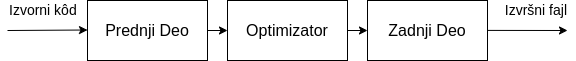
\includegraphics[width=0.8\textwidth]{assets/compiler_structure.png}
  \caption{Grafički prikaz strukture modernog kompajlera}
  \label{fig:compiler_structure}
\end{figure}

\section{Kompajlerske optimizacije}

% https://compileroptimizations.com/
% https://groups.seas.harvard.edu/courses/cs153/2019fa/lectures/Lec19-Optimization.pdf
% https://en.wikipedia.org/wiki/Constant_folding
% https://en.wikipedia.org/wiki/Optimizing_compiler

Kompajleri osim prevođenja izvornog koda do mašinskih instrukcija takođe mogu da ga modifikuju za bolje performanse sve dok se optimizovani k\^od ponaša isto kao originalni.
Performanse mogu da se odnose na vreme izvršavanja programa, memorijski prostor potreban prilikom izvršavanja ili memorijski prostor potreban za skladištenje izvršnog fajla.
U zavisnosti od faze kompilacije u kojoj se rade, optimizacije mogu biti nezavisne ili zavisne od ciljne arhitekture. % TODO cite
Nezavisne optimizacije rade za sve ciljne arhitekture i oslanjaju se na smanjivanje ukupnog broja operacija koje treba izvršiti.
Zavisne optimizacije iskorišćavaju detalje arhitekture kako bi podigli performanse.
To se ogleda u korišćenju instrukcija koje rade više operacija u isto vreme ili instrukcija koje rade brže od alternativnih.
Čest primer na arhitekturi \verb|x86_64| je zamena instrukcije \verb|mov eax, 0| sa instrukcijom \verb|xor eax, eax|.

Primeri nekih bitnih optimizacija su:
\begin{description}
  \item[Savijanje konstanti (eng.~{\em constant folding})] --- U programskom kodu se često javljaju konstantni matematički izrazi bez promenljivih. Oni mogu da budu direkno napisani u izvornom kodu, dobijeni pretprocesiranjem ili drugim optimizacijama itd. Kako izraz ne sadrži promenljive, nema razlog da se on evaluira za vreme izvršavanja svaki put već se to radi u vreme kompilacije.
  \item[Eliminacija mrtvog koda (eng.~{\em dead code elimination})] --- Statičkom analizom je moguće u specijalnim slučajevima utvrditi da se neki deo programa nikada neće izvrsiti. Brisanjem tog koda štedi se memorija, ubrzava proces kompilacije i može da se ubrza vreme izvršavanja zbog bolje organizacije keš memorije.
  \item[Globalna numeracija vrednosti (eng.~{\em global value numbering})] --- Neki izrazi ili delovi izraza se mogu javiti na više mesta u kratkom rasponu. Ukoliko su izračunati jednom, nije potrebno računati ih ponovo ispočetka već je moguće obezbediti da prethodni rezultat ostane dostupan u memoriji dok nije ponovo potreban.
  \item[Razmotavanje petlji (eng.~{\em loop unrolling})] --- Izvršavanje petlji sa kratkim telom dovodi do velikog broja skokova u maloj količini vremena. Skokovi su skupa instrukcija i njihovim smanjenjem mogu znatno da se povećaju performanse programa. Razmotavanje se radi tako što se telo petlje ponovi više puta u jednoj iteraciji i broj iteracija se isti broj puta smanji. Ovo je moguće samo u posebnim situacijama kada kompajler ima dovoljno informacija o načinu izvršavanja petlje.
\end{description}

% objasnjenje odnos O0, O1, O2, O3, Os, Oz (/Od, /O1, /O2, /Os)
% https://gcc.gnu.org/onlinedocs/gcc/Optimize-Options.html
% https://learn.microsoft.com/en-us/cpp/build/reference/o-options-optimize-code?view=msvc-170
% https://discourse.llvm.org/t/compiling-for-size/65415/6
% https://stackoverflow.com/questions/45608392/what-do-the-optimization-levels-os-and-oz-do-in-rustc

% TODO ovo nije tacno za MSVC
Postoji nekoliko nivoa optimizacije koji se mogu podesiti u prilikom poziva kompajlera.
Izbor nivoa određuje koje optimizacije treba da se izvrše.
Način odabira i nivoi optimizacije su drugačiji na različitim kompajlerima.
Na kompajlerima \verb|gcc| i \verb|clang| korisnik može da izabere nivo tako što prosledi zastavicu \verb|-O| iza koje se javlja neki od karaktera 0, 1, 2, 3 ili s\footnote{Ovo nije potpuna lista. Postoje nivoi koji nisu navedeni.}.
\verb|O0| je podrazumevani nivo ukoliko nijedan drugi nije naveden i označava da se k\^od uopšte ne optimizuje.
Ovaj režim se koristi za pravljenje debag verzija programa.
Više reči o tome će biti u poglavlju \ref{sec:informacije_za_debagovanje}.
\verb|O1| i \verb|O2| redom uključuju sve veći broj optimizacija podrazumevano da one drastično ne povaćavaju memorijsku složenost programa.
\verb|O3| ja najveći nivo optimizacije vremena izvršavanja.
On podrazumeva sve što se koristi u \verb|O2|, ali uključuje i optimizacije koje mogu da znatno povećaju memorijsko zauzeće programa.
Isporučene verzije programa se često kompajliraju na ovaj način.
Sa druge strane \verb|Os| nivo takođe podrazumeva sve optimizacije iz \verb|O2| ali dodatno i optimizacije koje smanjuju memorijsko zauzeće na uštrb vremena izvršavanja.
Ovaj nivo se koristi za uređaje sa ugrađenim računarom (eng.~{\em embedded devices}) koji imaju malu količinu memorije.

\section{Kompajler LLVM}

% https://llvm.org/
% https://en.wikipedia.org/wiki/LLVM
% The Architecture Of Open Source Applications - Chap 11
% https://aosabook.org/en/v1/llvm.html
% LLVM Essentials - Chapter 1
% https://www.prevodioci.matf.bg.ac.rs/kk/2020/predavanja/03_llvm_text.pdf
% https://www.prevodioci.matf.bg.ac.rs/KonstrukcijaKompilatora.html#2_tab

Projekat LLVM započet je 2000. godine na Univerzitetu Ilinois od strane Krisa Latnera. Ubrzo se projektu pridružio i njegov mentor Vikram Adve.
Cilj projekta je bio proučavanje tehnika kompajliranja u SSA obliku (eng.~{\em Static Single Assignment}) koje podržavaju statičku i dinamičku kompilaciju proizvoljnih programskih jezika.
Inicijalno, naziv LLVM je bio akronim za "virutelna mašina niskog nivoa" (eng.~{\em Low Level Virtual Machine}).
Od tada akronim se više ne koristi, ali je ime ostalo nepromenjeno.
Danas, projekat pokriva veliki broj biblioteka i alata koji se koriste za komercijalne i projekte otvorenog koda \cite{llvm}.
Svaki deo projekta je dizajniran kao biblioteka tako da se može ponovo upotrebiti za implementiranje drugih alata.
Celokupan izvorni k\^od je javno dostupan na servisu GitHub. % TODO link
Prednost pristupu otvorenog koda je da svako ko želi da poboljša k\^od ili ispravi neku grešku može to da učini.
Velika zajednica se formirala oko projekta što je znatno doprinelo njegovoj popularnosti.
Mnoge firme koriste svoje verzije kompajlera LLVM bilo za podršku neke arhitekture ili kao osnovu za novi programski jezik. % TODO cite
% Jezik Rust se oslanja na LLVM midle-backend

% Potprojekti znacajni za ovaj rad su: LLVM, Clang i LLDB
Glavnu komponentu projekta LLVM čini kolekcija biblioteka u okviru istoimenog potprojekta.
One implementiraju optimizator i zadnji deo kompajlera i koriste se od strane većine ostalih alata.
Drugi bitan potprojekat je clang. On implementira prednji deo kompajlera za jezike C, C++ i Objective-C.
LLVM implementira i svoj debager koji se zove LLDB. Više reči o njemu će biti u glavi \ref{sec:lldb}.
Postoji još veliki broj biblioteka i pomoćnih alata koji nisu pomenuti zato što nisu predmet ovog rada.

Kompajler LLVM je relativno nov u odnosu na druge popularne kompajlere i prati moderniji dizajn.
Za razliku od kompajlera GCC \cite{gcc}, koji je napisan u jeziku C i ima monolitnu strukturu, LLVM uživa u pogodnostima koje nudi jezik C++ pritom koristeći modularnu arhitekturu.
Dok je najveći deo projekta napisan u programskom jeziku C++, postoji interfejs za povezivanje sa jezicima C i Python.

Implementacija kompajlera LLVM prati opštu strukturu kompajlera prikazanu u poglavlju \ref{sec:compiler_structure} \cite{brown2011architecture}.
% slika alati koji prevode u svakom koraku kompilacije
Korake kompilacije izvršavaju različiti alati.
Odnos različitih reprezentacija koje program ima u toku kompilacije i alata koji konvertuju iz jedne reprezantacije u drugu je prikazan na slici \ref{fig:llvm_compile_tools}.
U nastavku će biti opisani redom prednji, srednji i zadnji deo LLVM kompajlera sa fokusom na poslednja dva kako su oni bitniji za ovaj rad.

\begin{figure}[!ht]
  \centering
  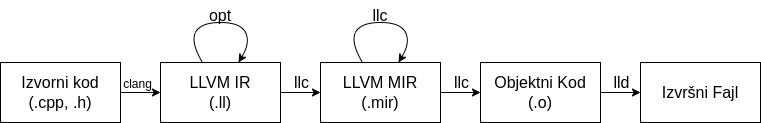
\includegraphics[width=\textwidth]{assets/llvm_compile_tools.png}
  \caption{Grafički prikaz reprezentacija koda prilikom kompilacije kompajlerom LLVM i alata koji se koriste za konverziju između njih}
  \label{fig:llvm_compile_tools}
\end{figure}


\subsection{Prednji deo}

Projekat LLVM sadrži vise različitih prednjih delova kompajlera.
Druge organizacije i firme takođe proizvode i održavaju prednje delove kompajlera LLVM za svoje jezike.
Iz tog razloga, LLVM podržava veliki broj programskih jezika koji uključuju C, C++, Objectve-C, Fortran, Haskell, Swift i druge.
Prednji deo za programske jezike C i C++ koji su fokus ovog rada naziva se Clang.

Postoji nekoliko značenja termina Clang.
Može se smatrati da je to prednji deo kompajlera, kao u skladu sa prethodnim korišćenjem izraza, zatim se može podrazumevati da je to alat koji upravlja celim procesom kompilacije ili može da bude biblioteka koja implementira funkcionalnost prednjeg dela kompajlera.
U okviru rada se podrazumeva prva interpretacija.

Funkcija ovog dela kompajlera je da izvorni k\^od, u ovom slučaju napisan u jezicima C ili C++ prevede u LLVM međureprezentaciju \cite{lopes2014llvmcorelibs}.
Usput se izvršavaju sve provere ispravnosti izvornog koda i prikazuju se greške i upozorenja korisniku.
Program se detaljno analizira iz nekoliko koraka i pritom dolazi do transformacija izvornog koda.

Prvo se prepoznaju osnovne jedinice gramatike programskog jezika, odnosno lekseme.
Lekseme se pretvaraju u različite tipove tokena u zavisnosti od toga šta označavaju.
Na primer za ključne reči programskog jezika postoje različite vrste tokena, dok svi identifikatori imaju isti tip tokena.
% Mnogo je lakše i brže raditi operacije nad tokenima nego u tekstualnom obliku.
Tokeni osim tipa imaju i informacije o opsegu koji zauzimaju u izvornom kodu pomoću kog se može pristupiti njihovom tekstu.
% Na ovaj način se ispisuju dijagnostičke poruke

Nad nizom tokena se radi sintaksna analiza ili parsiranje u skladu sa pravilima gramatike jezika.
Ta pravila se zadaju korišćenjem kontekstno-slobodne gramatike.
Primenom pravila gradi se sintaksno stablo gde unutrašnji čvorovi predstavljaju operacije a njihova deca su argumenti.
Parsiranje utvrđuje da li program ima ispravnu strukturu ali ne proverava da li taj program ima smisao.
To je zadatak semantičke analize.

Program može da ima dobru strukturu, ali da nema validno značenje.
Prolaskom kroz sintaksno stablo se prikupljaju informacije o funkcijama, promenljivima i drugim objektima i smeštaju se u tabelu simbola.
Korišćenjem te tabele proverava se ispravnost sintaksnog stabla.
Primer provere koja se vrši na ovom nivou je da li su promenljive deklarisane pre njihove upotrebe.
Rezultat svih ovih analiza je program u obliku apstraktnog sintaksnog stabla (eng.~{\em Abstract Syntax Tree, AST}).

U biblioteci Clang parsiranje i semantička analiza su usko povezani, a lekser se poziva po potrebi od strane parsera \cite{stulova2019overview}.
Bitan deo leksera čini pretprocesor koji izvšava direktive poput \verb|#include| i \verb|#define|.
Prilikom primene pravila gramatike parser zahteva tokene od leksera i delegira posao kreiranja sintaksnog stabla semantičkom analizatoru.
Ukoliko se pronađe greška u bilo kojoj analizi, program se ne moze kompajlirati i poruka o razlogu se vraća korisniku.
% Primer clang AST?
U suprotnom, obilaskom apstraktnog sintaksnog stabla generiše se LLVM međukod.
Komanda za prevođenje programa do LLVM međukoda prikazana je u listingu \ref{lst:clang_command}.

% primer clang komanda
\begin{figure}[!ht]
\begin{minted}[]{text}
  clang -S -emit-llvm -o output.ll input.c
\end{minted}
\caption{Komanda za kompilaciju izvornog koda do neoptimizovanog LLVM međukoda}
\label{lst:clang_command}
\end{figure}

Ukoliko se program uspešno prevede do međukoda, onda je izvorni k\^od validan za jezik u kome je napisan.
Još uvek je moguće da dođe do greške prilikom povezivanja zbog nepostojećih definicija nekih funkcija, klasa ili simbola, ali će kompilacija do asemblerskog ili objektnog koda biti uspešna.
Naravno, činjenica da se program kompajlira ne znači da on radi ono što je programer zamislio niti da će se program uvek uspešno završiti.

\subsection{Optimizator}

% https://llvm.org/docs/LangRef.html

% Optimizator - LLVM IR
Prednji deo prevodi izvorni k\^od u LLVM mašinski nezavisan međukod.
U terminologiji se koristi skraćenica IR (eng.~{\em Intermediate Representation}).
Izbor reprezentacije međukoda je veoma bitan kada kompajler treba da podrži i više programskih jezika i više ciljnih arhitektura.
On treba da je na dovoljno visokom nivou da ne zavisi od arhitekture i u isto vreme na dovoljno niskom nivou da ne zavisi od prgramskog jezika \cite{sarda2015llvm_essentials}.

LLVM međukod je u SSA obliku \cite{rastello2022ssa}.
To znači da je svakoj promenljivoj vrednost dodeljena samo jednom i da svakoj upotrebi promenljive prethodi njena definicija.
Ovaj oblik je izabran zato što je pogodan za izvršavanje optimizacija.

% Struktura LLVM IR fajla
U listingu \ref{lst:llvm_ir_example} je dat primer LLVM međukoda za program prikazan u listingu \ref{lst:ir_c_example}.
Kompletan pregled jezika LLVM IR dostupan je na internetu \cite{llvmlangref}.

\begin{figure}[!ht]
\begin{minted}[fontsize=\footnotesize,breaklines,linenos]{c}
#include <stdio.h>

int main() {
	int x;
	scanf("%d", &x);
	if (x % 2 == 0)
		printf("Hello, World!");
	return 0;
}
\end{minted}
\caption{C program napravljen za istraživanje strukture LLVM međukoda}
\label{lst:ir_c_example}
\end{figure}

% Primer IR koda
% clang -S -emit-llvm helloworld.c -o helloworld.ll
\begin{figure}[!ht]
\begin{minted}[fontsize=\footnotesize,breaklines,linenos]{llvm}
; ModuleID = 'helloworld.c'
source_filename = "helloworld.c"
target datalayout = "e-m:e-p270:32:32-p271:32:32-p272:64:64-i64:64-f80:128-n8:16:32:64-S128"
target triple = "x86_64-unknown-linux-gnu"

@.str = private unnamed_addr constant [3 x i8] c"%d\00", align 1
@.str.1 = private unnamed_addr constant [14 x i8] c"Hello, World!\00", align 1

; Function Attrs: noinline nounwind optnone uwtable
define dso_local i32 @main() #0 {
  %1 = alloca i32, align 4
  %2 = alloca i32, align 4
  store i32 0, ptr %1, align 4
  %3 = call i32 (ptr, ...) @__isoc99_scanf(ptr noundef @.str, ptr noundef %2)
  %4 = load i32, ptr %2, align 4
  %5 = srem i32 %4, 2
  %6 = icmp eq i32 %5, 0
  br i1 %6, label %7, label %9

7:                                                ; preds = %0
  %8 = call i32 (ptr, ...) @printf(ptr noundef @.str.1)
  br label %9

9:                                                ; preds = %7, %0
  ret i32 0
}

declare dso_local i32 @__isoc99_scanf(ptr noundef, ...) #1

declare dso_local i32 @printf(ptr noundef, ...) #1

...

!llvm.module.flags = !{!0, !1, !2, !3, !4}
!llvm.ident = !{!5}

!0 = !{i32 1, !"wchar_size", i32 4}
!1 = !{i32 7, !"PIC Level", i32 2}
!2 = !{i32 7, !"PIE Level", i32 2}
!3 = !{i32 7, !"uwtable", i32 2}
!4 = !{i32 7, !"frame-pointer", i32 2}
!5 = !{!"clang version 16.0.0"}
\end{minted}
\caption{Primer LLVM međukoda}
\label{lst:llvm_ir_example}
\end{figure}

Svaki fajl sa LLVM međukodom čuva informacije o jednom modulu.
Na početku fajla se nalazi ime fajla u kojem se nalazi izvorni k\^od, informacije o načinu zapisa podataka i naziv ciljne arhitekture.
U nastavku su globalne promenljive i funkcije.
One se prepoznaju po tome što im imena imaju prefiks '@'.

Svaka funkcija se sastoji od niza osnovnih blokova (eng.~{\em basic blocks}), a svaki blok od niza instrukcija.
Osnovni blok je jedinica čije instrukcije se uvek linearno izvršavaju. Ako se uđe u osnovni blok on će se uvek izvršiti do kraja \cite{aho2006compilers}. 
Dakle instrukcije grananja smeju i moraju da se pojave na kraju bloka.
Granice osnovnih blokova su ozačene kao labele u jeziku C.
Takođe, početak funkcije započinje prvi osnovni blok i kraj funkcije završava poslednji blok.

U okviru funkcije lokalne promenljive su zamenjene virtuelnim registrima.
Identifikatori virtuelnih registara počinju karakterom '\%'.
Zbog SSA oblika, svakom od njih se može dodeliti vrednost tačno jednom.
Smatra se da tih registara ima neograničen broj.

Instrukcije se sastoje od naziva (\verb|alloca|, \verb|call|, \verb|icmp|, ...), tipa (\verb|i32|, \verb|float|, \verb|label|, ...) i operanada.
Ukoliko instrukcija vraća vrednost, on se smešta u novi virtuelni registar.
Dodatne informacije o instrukcijama i globalnim objektima se čuvaju u vidu metapodataka.
Oni se mogu prepoznati po tome što počinju karakterom '!'.
Između ostalog, oni se koriste za informacije za debagovanje.
Vise reči o primeni metapodataka će biti u glavi \ref{sec:informacije_za_debagovanje}.

Optimizacije su implementirane u vidu prolaza (eng.~{\em pass}) koji obrađuju modul, funkciju ili petlju.
Prolazi nasleđuju apstraktnu klasu \verb|PassInfoMixin| i implementiraju funkciju \verb|run| sa argumentima za odgovarajuću jedinicu obrade.
Oni se dele na analize i transformacije.
Analize prikupljaju podatke dok transformacije koriste te podatke kako bi izmenili k\^od.
Transformacija zahteva različite vrste analiza i može da ih poništi ako više ne važe posle promene koda.

Optimizovanje programa se radi inkrementalno.
Program dobijen kao izlaz iz jedne optimizacije postaje ulaz sledećoj optimizaciji.
Dakle konačan program zavisi od redosleda izvršavanja optimizacija.
Loš redosled može da rezultuje znatno lošijim performansama izvršnog fajla.
% Zbog toga optimizacije su pažljivo poređane.
Svaki nivo optimizacije propisuje koje optimizacije treba da budu primenjene i kojim redosledom.

% opt alat
Za primenu optimizacija na LLVM IR fajlu se koristi alat \verb|opt|.
On prima imena optimizacija koje treba da pokrene i fajl sa ispravnim IR programom koji ga optimizuje.
Takođe moguće je pokretanje korisnički napisanih prolaza učitanih kao dinamičke biblioteke \cite{pandey2017cookbook}.
Primer korišćenja alata je prikazan u listingu \ref{lst:opt_command}.
% primer opt komanda
\begin{figure}[!ht]
\begin{minted}[]{text}
  opt -passes="mem2reg,instnamer" -o output.ll input.ll
\end{minted}
\caption{Komanda za optimizovanje LLVM međukoda koristeći optimizacije \texttt{mem2reg} i \texttt{instnamer}}
\label{lst:opt_command}
\end{figure}

\subsection{Zadnji deo}

% IR -> Instruction Selection -> Instructio Scheduling -> Passes -> Register Allocation -> Passes -> Instruction Scheduling -> Passes -> Code Emission
% Isel: IR -> MIR, legalizacija instrukcija, alocirani registri, nije ih vise beskonacno, pre-RA/post-RA scheduling
% scheduling: rasporedjivanje instrukcija

% Zadnji deo - Instruction selection, SelectionDAG, MIR, AsmPrinter
Pre generisanja mašinskog koda, postoji još jedna, mašinski zavisna, interna reprezentacija.
U terminologija projekta LLVM, ona se naziva MIR (eng.~{\em Machine Intermediate Representation}).
Ona je dosta bliža ciljnoj arhitekturi i sastoji se od konkretnih instrukcija za tu arhitekturu.
MIR k\^od se zapisuje u formatu YAML \cite{yaml}.
Odlike funkcija poput imena, mesta poziva itd. su opisane atributima formata YAML.
Tela funckija se takođe nalaze u okviru atributa, serijalizovani u obliku niske.
Struktura instrukcija je slična kao za IR k\^od.
Najveće razlike su u tome što su intrukcije vezane za konkretnu arhitekturu i virtuelni registri su zamenjeni pravim registrima.
Kompletan pregled jezika dostupan je u okviru dokumentacije projekta LLVM \cite{mirlangref}.

Veliki i kompleksan korak u prevođenju koda je spuštanje sa mašinski nezavisne na mašinski zavisnu reprezentaciju.
Taj korak se naziva izbor instrukcija (eng.~{\em Instruction Selection}).
Postoje tri implementacije izbora instrukcija \cite{nacke2021learn}:
\begin{description}
  % https://llvm.org/docs/CodeGenerator.html#instruction-selection-section
  \item[\texttt{SelectionDAG}] --- Podrazumevana implementacija izbora instrukcija na većini arhitektura. Koristi grafovsku reprezantaciju programa i algoritme za uparivanje čvorova i različite vrste obilaska grafa \cite{lopes2014llvmcorelibs}.
  % https://llvm.org/docs/GlobalISel/index.html
  \item[\texttt{GlobalIsel}] --- Nova implementacija izbora instrukcija sa modularnim dizajnom, poboljšanim performansama i mogućnosti da optimizuje veći deo k\^oda. Trenutno nije završena implementacija, ali se planira da u budućnosti zameni \verb|SelectionDAG|.
  % "Fast" instruction selection is designed to emit very poor code quickly.
  % Also, it is not designed to be able to do much lowering, so most illegal
  % types (e.g. i64 on 32-bit targets) and operations are not supported.  It is
  % also not intended to be able to do much optimization, except in a few cases
  % where doing optimizations reduces overall compile time.  For example, folding
  % constants into immediate fields is often done, because it's cheap and it
  % reduces the number of instructions later phases have to examine.
  \item[\texttt{FastIsel}] --- Pristup izboru instrukcija koji radi veoma brzo, ali generiše neoptimizovan k\^od. Ne podržava spuštanje svih instrukcija i u tim situacijama se oslanja na \verb|SelectionDAG|.
\end{description}
Ovaj rad se fokusira na implementaciju \verb|SelectionDAG| zbog svoje stabilnosti i zato što je podrazumevana za arhitekturu \verb|x86_64|.

% SelectionDAG faze: IR -> Build SelectionDAG (w/ TargetLowering) -> combines and legalizations -> Isel Proper (DAG-to-DAG pattern matching)
Implementacija \verb|SelectionDAG| je dobla ime po načinu reprezentacije koda za vreme izbora instrukcija.
Naime, odgovarajuća klasa se takođe zove \verb|SelectionDAG|.
Osnovni blokovi programa su predstavljeni usmerenim acikličkim grafovima (eng.~{\em Directed Acyclic Graphs}).
Čvorovi tog grafa su instrukcije koje imaju tip \verb|SDNode|, a grane su različite zavisnosti koje postoje između instrukcija.
Postoje dva posebna čvora: ulazni čvor i koren.
Ulazni čvor obeležava početak osnovnog bloka i služi samo za postavljanje veza.
Sa druge strane, koren označava kraj bloka. Na kraju obrade je vezan za poslednju instrukciju osnovnog bloka.
% tipovi veza: zavisnost podataka, lančane zavisnosti, zalepljene zavisnosti

Konstrukcija grafa se radi prolaskom kroz LLVM međukod uz pomoć klase \verb|SelectionDAGBuilder| koja implementira obrazac "posetilac" (eng.~{\em visitor pattern}) \cite{gamma1995design}. 
Za svaku instrukciju se kreira čvor na osnovu njenog koda operacije.
Konstrukcija čvora se radi direktno u klasi \verb|SelectionDAG|.
Veze se kreiraju kada neki čvor koristi izlaznu vrednost drugog čvora.
Tip te vrednosti određuje tip veze.
% Program sastoji od niza \verb|SelectionDAG| struktura.

% combine and legalize
Prethodno konstruisan graf nije pogodan za spuštanje instrukcija i nad njim se vrše dodatne transformacije.
On se dodatno optimizuje zamenom grupe povezanih čvorova sa jednostavnijim grupama uz pomoć algoritama za uparivanje stabala.
Te optimizacije mogu da budu i mašinski nezavisne i zavisne.
Graf takođe može da sadrži nepodržane tipove i operacije za ciljnu arhitekturu.
Njih je potrebno zameniti odgovarajućim podržanim varijantama.
Ove transformacije se zovu legalizacija tipova i operacija.
Način legalizacije zavisi od arhitekture i implementiran je u odgovarajućim \verb|TargetLowering| klasama.
Prolazi optimizacije i legalizacije se rade nekoliko puta u određenom redosledu i rezultuju grafom spremnim za spuštanje instrukcija.

% isel proper / dag-to-dag
Proces spuštanja instrukcija kada su sve potrebne pripreme izvršene je prilično jednostavan.
Kao i prilikom optimizacija, algoritam se zasniva na uparivanju čvorova.
Čvorovi svake \verb|SelectionDAG| strukture traže svoj pandan za ciljnu arhitekturu.
Arhitektura definiše ta uparivanja u svojoj podklasi klase \verb|SelectionDAGISel|.
Ona definiše funkciju \verb|Select| koja prima objekat tipa \verb|SDNode| i vraća čvor sa mašinski zavisnim kodom operacije.
U ovom koraku se ne zamenjuju baš svi čvorovi već neki prolaze u sledeću fazu.

% Instruction scheduling and register allocation
Poslednji trag LLVM međukoda koji je opstao u programu a da je potrebno da se eliminiše su virutelni registri.
U toku izvršavanja program će imati ograničen broj registara i ne može svaki od njih da se koristi za svaku operaciju.
Dodeljivanje registara je korak kada se virtuelni registri zamenjuju konkretnim registrima za ciljnu arhitekturu.
Po potrebi dodaju se nove instrukcije za čuvanje i učitavanje vrednosti registara.
Dobijeni \verb|SelectionDAG| predstavlja instrukcije potpuno ispravnog MIR programa.
% Ostalo je još da se te instrukcije rasporede u linearni redosled.
% Graf nameće neke uslove za to koje instrukcije zavise od drugih, ali još uvek postoji sloboda u odabiru instrukcija koje nisu međusobno povezane.
% Iako je bilo koji od mogućih rasporeda ispravan, postoje rasporedi koji pružaju bolje performanse.
% Razlog za to je što raspored utiče na paralelizaciju na nivou instrukcija.
% Koristeći podatke o ciljnoj mašini, instrukcije se biraju na osnovu heuristika za poboljšanje performansi.
% Ovo rezultuje kodom u MIR obliku.
Ostalo je još da se one rasporede u linearni redosled uz poštovanje zavisnosti između čvorova.
Ovo rezultuje kodom u MIR obliku.

% Na kraju spuštanja instrukcija program je još uvek u obliku grafa.
% Te instrukcije je potrebno rasporediti u niz.
% Graf nameće neke uslove za to koje instrukcije zavise od drugih, ali još uvek postoji sloboda u odabiru instrukcija koje nisu međusobno povezane.
% Iako je bilo koji od mogućih rasporeda ispravan, postoje rasporedi koji pružaju bolje performanse.
% % raspored treba da obezbedi sto bolju paralelizaciju na nivou instrukcija
% Razlog za to je što raspored utiče na dodeljivanje registara i paralelizaciju na nivou instrukcija.
% Dodeljivanje registara je korak kada virtuelni registri iz IR oblika zamenjuju konkretne registre za ciljnu arhitekturu.
% Po potrebi dodaju se nove instrukcije za čuvanje i učitavanje vrednosti registara.
% % Raspoređivanje se vrši dva puta, pre i posle dodeljivanja registara.
% Koristeći podatke o ciljnoj mašini, instrukcije se biraju na osnovu heuristika za poboljšanje performansi.
% Ovo rezultuje kodom u MIR obliku.

% MIR prolazi
Kao kod mašinski nezavisnog međukoda i na ovom nivou postoje optimizacioni prolazi.
Optimizacije na ovom nivou su vezane za ciljnu arhitekturu.
Svi mašinski zavisni prolazi nasleđuju klasu \verb|MachineFunctionPass| i implementiraju funkciju \verb|runOnMachineFunction| koja se poziva za svaku funkciju u izvornom kodu.
Način izvršavanja prolaza je sličan kao za mašinski nezavisan međukod.
Oni se izvršavaju iterativno u unapred zadatom redosledu.

% Code emission: MachineInstr -> MCInst
Poslednji prolaz na MIR kodu je \verb|AsmPrinter| koji emituje asmeblerski ili objektni k\^od za ciljnu arhitekturu.
% Usput se instrukcije prevode u novu reprezentaciju, \verb|MCInst|.
Na ovom mestu se završava zadatak kompajlera.
Dalje, ukoliko je emitovan asemblerski k\^od on se prevodi do objektnog koristeći asmebler.
Objektni k\^od se povezuje sa sistemskim i korisničkim bibliotekama i drugim objektnim kodom pomoću povezivača (eng.~{\em linker}) i dobija se izvršni fajl.

Alat koji obavlja posao zadnjeg dela kompajlera je \verb|llc|.
Njemu se opciono zadaje vrsta izlaza (asemblerski ili objektni k\^od) i nivo optimizacije.
Bitan parametar koji \verb|llc| prihvata je ciljna arhitektura.
% https://www.flother.is/til/llvm-target-triple/
Ona se zadaje argumentom \verb|-mtriple| i vrednosti u vidu niske koja sadrži arhitekturu, proizvođača, operativni sistem i okruženje.
% TODO: odabir optimizacija, print after all
Komanda za prevođenje mašinski nezavisnog međukoda do asemblerskog fajla za arhitekturu \verb|x86_64| i operativni sistem Linux je prikazana u listingu \ref{lst:llc_command}.

% primer llc komanda
\begin{figure}[!ht]
  \begin{minted}[breaklines]{text}
    llc -filetype=asm -mtriple="x86_64-unknown-linux-gnu" -o output.s input.ll
  \end{minted}
  \caption{Komanda za prevođenje LLVM međukoda do asemblerskog koda za x64 arhitekturu}
  \label{lst:llc_command}
\end{figure}


\chapter{Debageri}
\label{sec:debuggers}

% https://en.wikipedia.org/wiki/Debugging
% https://eli.thegreenplace.net/2011/01/23/how-debuggers-work-part-1

% opste o greskama, procesu razvoja softvera
% print debagovanje i debageri
Prilikom programiranja bilo kog većeg projekta, neminovno je da će doći do propusta.
% Ti propusti se popularno nazivaju bagovi.
Propusti se odnose na bilo kakvo ponašanje programa koje nije u skladu sa namerom programera.
% To može da bude na primer nekonzistentnost u korisničkom interfejsu, greška u nekom algoritmu ili 
U zavisnosti od komponente programa u kojoj se propust ispoljava, posledice mogu da budu više ili manje ozbiljne.
Na primer, greška u korisničkom interfejsu ima dosta manje posledice od greške u sistemu obrade novca u banci.
Svakako, svi primećeni propusti trebaju biti popravljeni pre objavljivanja nove verzije softvera.

% Debagovanje je proces pronalaženja, reprodukovanja, analiziranja i popravljanja grešaka u programu.
Proces pronalaženja, reprodukovanja, analiziranja i popravljanja grešaka u programu naziva se debagovanje.
% Jedan od najtežih koraka tog procesa je određivanje problematičnog dela koda, dok je rešavanje problema najlakši deo.
% Postoji nekoliko načina debagovanja.
Jedan od osnovnih načina je debagovanje štampanjem (eng.~{\em print debugging}).
Ono podrazumeva izmenu izvornog koda tako da ispisuje poruke i vrednosti promenljivih u glavnim koracima dela koda za koje programer smatra da su razlog za postojanje greške.
Za sitnije greške ovo je sasvim prihvatljiv način za njihovo rešavanje.
Mana tog pristupa je potreba za ponovnom kompilacijom celog programa svaki put kada se dodaje ili menja ispis.
Kompilacija velikih projekata može da dugo traje, tako da se ovaj pristup ne isplati uvek.
Alternativa je korišćenje posebnog alata namenjenog za ovu situaciju.

Debager je softverski alat koji olakšava proces debagovanja.
On pruža interaktivan vid izvršavanja programa gde korisnik zadaje komande za izvršavanje programa i proveru vrednosti promenljivih.
Umesto izmene izvornog koda, debager direktno ispituje i modifikuje program dok se izvršava.
%Umesto izmene izvornog koda, debager
On uz pomoć operativnog sistema dobija potpunu kontrolu nad izvršavanjem programa.
To mu daje pristup za čitanje i pisanje cele memorije programa dok se izvršava, uključujući i instrukcije koje će se izvršiti.
Na taj način debager može i da kotroliše tok izvršavanja tog programa.
% mogucnosti debagera
Neke od funkcionalnosti debagera su: % cite
\begin{itemize}
  \item Evaluiranje vrednosti izraza --- Kada je proces zaustavljen na nekom mestu u kodu, korisnik može da proveri vrednosti promenljivih u tom trenutku. Neki debageri osim toga podržavaju i izračunavanje proizvoljnih izraza koji uključuju promenljive i funkcije programa koji se debaguje.
  \item Izvršavanje korak po korak --- Najčešći i najjednostavniji vid kretanja kroz program. Omogućava kontrolisano izvršavanje samo određenog dela koda. Korak može da označava jednu instrukciju, jedan red ili jednu funkciju. % TODO expand
  \item Postavljanje tačaka prekida --- Ukoliko programer već naslućuje koji deo koda izaziva problem, on ne želi da izvršava korak po korak program dok se ne dostigne taj deo. Umesto toga može da postavi tačku prekida (eng.~{\em breakpoint}) na to mesto i pusti program da se sam izvršava. Svaki put kada se dostigne tačka prekida proces će biti zaustavljen. % Postoje i načini za zadavanje uslova u kojim situacijama 
  \item Praćenje vrednosti promenljivih --- Neki bagovi su izazvani neočekivanom promenom vrednosti neke promenljive. Pogodan način za otkrivanje trenutka kada se to desi je postavljanjem tačke prekida nad podatkom (eng.~{\em watchpoint}). Promenom vrednosti na toj adresi će se zaustaviti proces i kontrola se vratiti korisniku.
  % \item Pregled vrednosti u memoriji --- 
  \item Pregled stek okvira --- Pronalazak mesta gde je greška ispoljena nije uvek dovoljno da se odredi gde ona nastaje. Taj deo koda se možda poziva sa više mesta i potrebno je odrediti koji od njih je izazvao problem. Pregledom stek okvira korisnik dobija uvid u istoriju poziva funkcija od početne funkcije.
  \item Izvršavanje programa unazad --- Nekada korisnik uoči problem tek nekoliko koraka nakon što je on nastao. Napredni debageri imaju podršku za poništavanje izvršenih instrukcija. Programski brojač se pomera unazad i sva izmenjena memorija se vraća na prethodno stanje.
\end{itemize}
Najpoznatiji debageri za jezike C i C++ su \textit{GDB}, \textit{LLDB} i \textit{Microsoft Visual Studio Debugger}.

% Source level debugging
% Iako je debagovanje moguće na nivou mašinskih instrukcija, to nije mnogo praktično.
% Umesto toga debagovanje je pogodnije raditi na nivou izvornog koda (eng.~{Source Level Debugging}).

Tradicionalan način korišćenja debagera je putem komandne linije.
Sve operacije se izvršavaju zadavanjem komande u tekstualnom obliku u formatu koji debager propisuje.
Upotrebom komande za pokretanje dela ili celog programa korisnik više ne može da zadaje nove komande sve dok se prethodna komanda ne izvrši do kraja.
Problem sa ovim vidom upotrebe je što korisnik mora da napamet zna strukturu komandi ili da otvara dokumentaciju.
Drugi način za upotrebu debagera je pomoću integrisanih razvojnih okruženja (eng.~{\em integrated development environment}).
Mnoga okruženja ugrađuju debager u svoj grafički korisnički interfejs (eng.~{\em graphical user interface}).
Postojanje grafičkih elemenata olakšava posao korisniku zato što ne mora da memoriše sve komande.
Dovoljno je da pritisne odgovarajuće dugme ili na neki način izmeni neki drugi grafički element.
Ovo je najpogodniji način za nove korisnike da nauče da koriste debager.
Postoji i sredina između prethodna dva načina upotrebe u vidu tekstualnog korisničkog interfejsa (eng.~{\em textual user interface}).
Umesto odvojenog prozora, i dalje se koristi komanda linija, ali je ona napravljena tako da liči na grafičko okruženje.
Kako ne postoji podrška za kursor, komande se zadaju prečicama na tastaturi.

U nastavku će prvo biti objašnjen koncept informacija za debagovanje, a zatim će biti opisan format DWARF koji služi za zapisivanje tih informacija.
Na kraju poglavlja je predstavljen debager LLDB i neki ključni delovi njegove implementacije.

\section{Informacije za debagovanje}
\label{sec:informacije_za_debagovanje}

% https://blog.syrmia.com/posts/debag-informacije-i-optimizacije-kompajlera-llvm
% https://www.prevodioci.matf.bg.ac.rs/kk/2021/predavanja/gostujucePredavanje/DjordjeTodorovic_LLVM_DebagInformacije.pdf
% https://www.llvm.org/devmtg/2016-11/Slides/Kleckner-CodeViewInLLVM.pdf

% https://llvm.org/docs/SourceLevelDebugging.html
% https://www.llvm.org/docs/HowToUpdateDebugInfo.html

% Source level debugging
% Debagovanje radi na nivou izvornog koda, ali on nije vezan za krajnji program.
Za uspešno debagovanje programa na nivou izvornog koda (eng.~{source level debugging}) potrebna je podrška kompajlera da sačuva informacije o tom kodu do izvršnog fajla.
Pored mašinskog koda, kompajler takođe, ako mu je zatraženo, generiše i dodatne informacije koje se koriste za debagovanje.
Između ostalog, one uključuju mapiranja mašinskih instrukcija u lokacije u izvornom kodu, imena funkcija i promenjivih itd.
Sve te informacije zauzimaju dodatnu memoriju u krajnjem izvršnom fajlu i produžavaju vreme kompilacije.
Iz tog razloga, one se podrazmevano ne generišu, već je potrebno eksplicitno navesti kompajleru da treba to da uradi.
Kompajler LLVM generiše ove podatke dodavanjem zastavice \verb|-g| u okviru komande za kompilaciju.

% Generisanje i ocuvavanje debag informacija
Većina informacija za debagovanje nastaju u prednjem delu kompajlera, pošto je on zadužen za analiziranja izvornog koda, i prosleđuju se kroz ostale faze kompilacije gde se usput dopunjuju novim podacima kada oni postanu dostupni (npr. lokacije promenljivih za vreme izvršavanja). % do izvršnog fajla.
% Odnos optimizacija i debag informacija
Očuvanje informacija za debagovanje nailazi na problem kada se uključe kompajlerske optimizacije.
Prilikom primene optimizacija, informacije za debagovanje i dalje treba reflektuju izvorni kod, a ne njegovu optimizovanu verziju.
Što se više krajnji program razlikuje od izvornog koda postaje teže očuvati informacije, a nekada je to čak potpuno nemoguće.
% U slučaju da je moguće izabrati između nepotpunih informacija ili informacija koje ne odgovaraju u potpunosti izvornom kodu, bolje je izabrati prvu opciju.
% Prihvatljivije je nemati informacije za debagovanje nego imati netačne.
Ovo je jedan od najvećih izazova pisanja optimizacija.
Jednostavno rešenje je isključiti kompajlerske optimizacije prilikom debagovanja i ono može da bude pogodno za neke korisnike.
% To jeste dobro rešenje u situacijama kada je to moguće i praktično.
Ipak, postoje situacije kada je potrebno prevesti program sa optimizacijama.
Na primer u slučaju da se program kompajlira za računar sa malom količinom memorije gde ne može da se kompletno smesti ukoliko nije optimizovan za memoriju.
Drugi problem prevođenja bez optimizacija je što se program onda razlikuje od verzije koja se isporučuje klijentu i moguće je da se bag ispoljava samo u toj verziji.
Iz prethodno navedenih razloga se posebna pažnja prilikom pisanja optmizacija daje održavanju informacija za debagovanje.

Ove informacije se nalaza u posebnim delovima izvršnog fajla odvojenim od svega ostalog.
% Ove informacije se nalaze u posebnim segmentima, van uobičajenih segmenata (text, data, bss...).
Izvršni fajl je podeljen u nekoliko delova koji se nazivaju segmenti.
Najbitniji među njima su tekst segment gde se nalaze instrukcije programa, segment inicijalizovanih podataka i segment neinicijalizovanih podataka.
Pored njih mogu da postoje i drugi segmenti, na primer za podatke o razmotavanju steka u slučaju greške.
% ne smeju da menjaju kod koji se izvrsava
Informacije za debagovanje ne diraju nijedan od prethodnih segmenata već definišu nove kako ne bi uticali na postojeće podatke.
Broj i naziv novih segmenata zavisi od formata za zapisivanje informacija za debagovanje koji se koristi.
% Format propisuje način zapisivanja podataka i njihovog dekodiranja.
% Postoji više različitih formata za zapisivanje informacija za debagovanje.
Najpopularniji među njima su format CodeView za \textit{Windows} sisteme i format DWARF za sisteme UNIX tipa.

% Zasto postoje formati
% Mogucnost koriscenja razlicitih kombinacija kompajlera i debagera
Postojanje standardizovanih formata ima veliki značaj.
Ono omogućava korišćenje debagera nezavisno od kompajlera kojim je program preveden.
Bitno je samo da oba koriste isti format.
Ukoliko bi svaki kompajler pisao informacije za debagovanje u nekom ličnom (eng.~{propriatery}) formatu, on bi mogao da se koristi samo sa odgovarajućim debagerom.
Zbog standardizovanih formata, program preveden na primer kompajlerom GCC može da se debaguje debagerom LLDB.
% Iako moze da se zameni kompajler, ne mora da znaci da ce isti podaci biti generisani niti da ce ih debager u istoj meri korstiti
Iako koriste iste formate, ne mora da znači da će bilo koja dva debagera moći u potpunosti da iskoriste sve dostupne informacije za debagovanje ili da će ih korisiti na iste načine.

\section{Format DWARF}
\label{sec:dwarf}

% Introduction to the DWARF Debugging Format
% https://en.wikipedia.org/wiki/DWARF

\textit{DWARF} je standardizovan format za zapisivanje informacija za debagovanje.
Originalno je osmišljen da radi uz format ELF koji se koristi za biblioteke, izvršni i objektni k\^od, ali podržava i druge formate.
% Ime je dobio zato što je namenjen da se koristi uz format za izvršne fajlove i biblioteke, ELF, ali se može koristiti i uz druge formate.
Postoji podrška za programske jezike C, C++, Ada, Fortran i COBOL, ali je omogućeno proširenje i za druge jezike.
Ovaj format se koristi na UNIX sistemima što uključuje \textit{Linux} distribucije i \textit{macOS}.
Postojalo je nekoliko revizija standarda do sada, a trenutno je aktuelna verzija 5 koja će biti podrazumevana u nastavku rada.

Sve informacije za debagovanje su raspoređene u nove sekcije izvršnog fajla koje počinju prefiksom \verb|.debug_|.
Neke od najbitnijih su \cite{eager2012introduction_dwarf}:
\begin{itemize}
  \item \verb|.debug_info| --- Glavna sekcija za debagovanje. Sadrži skoro sve informacije o entitetima iz izvornog koda.
  \item \verb|.debug_line| --- Tabela adresa instrukcija u izvršnom fajlu i odgovarajućih lokacija u izvornom kodu. Takođe sadrži dodatne podatke o granicama prologa i epiloga funkcija.
  \item \verb|.debug_frame| --- Podaci o načinu razmotavanja stek okvira.
  \item \verb|.debug_loclists| --- Lokacije skladištenja promenljivih za vreme izvršavanja. Za jednu promenljivu može da postoji više lokacija na primer ako se promeni registar u kome je smeštena.
  % \item \verb|.debug_rnglists| --- Prekidni opsezi adresa. Koriste se iz \verb|.debug_info| sekcije kada opseg koji je potrebno opisati nije neprekidan.
  \item \verb|.debug_abbrev| --- Skraćenice za zapisivanje informacija u \verb|.debug_info| sekciji. Koristi se za kompresovanje podataka. % Umesto da se ispred svakog atributa napise njegov tip, ovde se definiše etiketa i redosled svih atributa u okviru jedinice i dodeljuje se skraćenica za zapis te jedinice.
  \item \verb|.debug_str| --- Tabela niski koje se koriste u \verb|.debug_info| sekciji.
\end{itemize}

% etikete i atributi
Podaci u sekciji \verb|.debug_info| su predstavljeni pomoću osnovnih jedinica (eng.~{\em Debug Information Entry, DIE}) organizovanih u drvoliku strukturu.
Svaka jedinica ima etiketu (eng.~{\em tag}) koja označava njen tip, dodatne informacije predstavljene atributima i može da ima druge jedinice kao decu.
Etikete i atributi imaju numeričku vrednost koja služi za zapisivanje u računaru i ime u obliku niske koje služi čoveku za lako čitanje podataka.
Standard propisuje validne etikete i atribute koje moraju da postoje za te etikete.
Ideja je da svaki entitet programskog jezika bude opisan na ovaj način.
U listingu \ref{lst:dwarf_variable} prikazan je primer opisa jedne promenljive.
Značenja prikazanih atributa su objašnjena kasnije u odeljku.
% Format je veoma kompresovan, što je neophodno za zapisivanje velike količine informacija kakvu imaju veliki projekti.
% Svi podaci se čuvaju kao numerički literali sa propisanim veličinama.

\begin{figure}[!ht]
\begin{minted}[]{text}
DW_TAG_variable
    DW_AT_location  (DW_OP_fbreg -8)
    DW_AT_name      ("x")
    DW_AT_decl_file ("/home/vladimir/Documents/example.c")
    DW_AT_decl_line (2)
    DW_AT_type      (0x00000052 "int")
\end{minted}
\caption{Primer DWARF jedinice koja opisuje promenljivu}
\label{lst:dwarf_variable}
\end{figure}

% Primeri etiketa i atributa
Etiketa označava neki entitet izvornog koda ili koncept programskog jezika.
Naziv etikete ima prefiks \verb|DW_TAG_| posle kog može da sledi oznaka proizvođača ako je u pitanju proširenje.
Neke od najbitnijih etiketa su:
\begin{itemize}
  \item \verb|DW_TAG_compile_unit| --- Predstavlja jednu kompilacionu jedinicu. Kao decu sadrži prostore imena (eng.~{\em namespace}), funkcije, globalne promenljive itd.
  \item \verb|DW_TAG_subprogram| --- Predstavlja jednu funkciju. Sadrži podatke o imenu, parametrima i opsegu funkcije u izvršnom fajlu, između ostalog.
  \item \verb|DW_TAG_call_site| --- Označava mesto poziva funkcije. Sadrži referencu na jedinicu \verb|DW_TAG_subprogram| za pozvanu funkciju i adresu povratka iz poziva.
  \item \verb|DW_TAG_variable| --- Opisuje jednu promenljivu. Ima informacije o njenom imenu, lokaciji u izvršnom fajlu i mestu deklaracije u izvršnom kodu.
  \item \verb|DW_TAG_base_type| --- Pruža informacije o osnovnim tipovima uključujući njihov način zapisa i veličinu. Postoje slične etikete za tipove nizova i niski.
\end{itemize}

Atributi opisuju svojstva objekata označenih etiketom uz koju stoje.
Isti atribut može imati više interpretacija u zavisnosti od etikete, ali jedan atribut se ne može ponavljati više puta u osnovnoj jedinici.
Redosled atributa unutar jedinice nije definisan i ne treba se oslanjati da će biti konzistentan.
Slično kao za etiketa, atribut počinje niskom \verb|DW_AT_| posle koje može da sledi oznaka proizvođača ako je u pitanju proširenje.
Neki od najbitnijih atributa su:
\begin{itemize}
  \item \verb|DW_AT_name| --- Može da opisuje ime funkcije, promenljive, labele itd.
  \item \verb|DW_AT_low_pc|, \verb|DW_AT_high_pc| --- Oba atributa zajedno opisuju opseg adresa. To može da bude opseg kompilacione jedinice, funkcije, postojanja promenljive itd. Ukoliko ne postoje informacije o obe granice, mogu se koristiti i odvojeno.
  \item \verb|DW_AT_decl_file| --- Fajl izvornog koda u kome je deklarisan objekat.
  \item \verb|DW_AT_decl_line| --- Red u izvornom kodu na kome je deklarisan objekat.
  \item \verb|DW_AT_decl_col| --- Kolona u izvornom kodu na kojoj je deklarisan objekat.
  \item \verb|DW_AT_type| --- Može da označava različite stvari u zavisnosti od konteksta. Najčešće je u pitanju tip koji ima neka promenljiva ili povratna vrednost funkcije. 
\end{itemize}

% DWARF expression?
% Postoji i podrška za izračunavanje vrednosti na osnovu vrednosti regisata i drugih promenljivih dostupnih u vreme izršavanja.
% Primena te funkcionalnosti je na primer izračunavanje vrednosti promenljivih koje su izoptimizovane.
% Na primer ukoliko debager ima informaciju da je vrednost te promenljive jednaka zbiru dva registra, to se može zapisati u okviru izraza i izračunati kada je potrebno.
% Implementirano je pomoću niza operacija koji deluju nad stekom vrednosti.

% Prosirivost
Bitna odlika formata DWARF je njegova proširivost.
Standard pruža način da se format dopuni novim etiketama i atributima od strane proizvođača kompajlera.
Razni alati mogu zatim da koriste te podatke kako bi poboljšali svoju funkcionalnost.
% To mogu biti debageri, 
% Alati koji koriste te podatke mogu da preskoče vrednosti koje ne razumeju, tako da se održava kompatibilnost sa svim alatima.
Sa druge strane, postojeći alati koji ne razumeju te podatke mogu samo da ih preskoče.
Na taj način se održava kompatibilnost sa postojećim alatima.
Slično važi za alate koji su napravljeni za starije verzije standarda.
% Bitno je da ne koristi vec rezervisana imena i vrednosti koje im odgovaraju
% Ko god želi da implementira svoje proširenje standarda može da osmisli svoje etikete i atribute.
Bitna stvar pilikom dodavanja etiketa i atributa je da im se dodele numeričke vrednosti koje nisu već deo standarda i poželjno bi bilo da se takođe ne koriste od strane drugih proizvođača kompajlera.
Raspon dozvoljenih vrednosti je dovoljno veliki da ne dođe do preklapanja vrednosti.
Kompajleri često koriste samo neki mali opseg za svoje potrebe.
% Da bi uvedeni podaci bili korisni potrebno je podržati ih u nekom alatu.

\section{Debager LLDB}
\label{sec:lldb}

% https://en.wikipedia.org/wiki/LLDB_(debugger)
% https://lldb.llvm.org/
% https://lldb.llvm.org/use/tutorial.html

% https://lldb.llvm.org/python_api/lldb.SBSymbolContext.html
% https://lldb.llvm.org/cpp_reference/classlldb__private_1_1SymbolContext.html#details
% https://lldb.llvm.org/cpp_reference/classlldb__private_1_1SymbolContextScope.html
% https://lldb.llvm.org/cpp_reference/classlldb__private_1_1StackFrame.html
% https://lldb.llvm.org/cpp_reference/classlldb__private_1_1Address.html

% LLDB je jedan od potprojekata koji se razvija kao deo projekta LLVM.
LLDB je debager koji se razvija kao deo projekta LLVM.
% It is built as a set of reusable components which extensively use existing libraries from LLVM, such as the Clang expression parser and LLVM disassembler
Napravljen je kao skup ponovo upotrebljivih komponenti koje ekstenzivno koriste biblioteke iz projekta LLVM kao što su parser izraza biblioteke clang ili disasembler biblioteke LLVM \cite{lldb}.
Podržava programske jezike C, C++ i Objective-C i dostupan na svim popularnim operativnim sistemima: \textit{Windows}, \textit{macOS} i \textit{Linux}.
LLDB je podrazumevani debager u integrisanom razvojnom okruženju \textit{Apple Xcode} i podržan je od strane drugih okruženja uključujući \textit{JetBrains CLion}, \textit{QtCreator}, \textit{Eclipse} i \textit{VSCode}.

% Komande
Primarni vid upotrebe alata LLDB je putem komandne linije.
Korisnik upravlja načinom izvršavanja debagovanog procesa tako što zadaje komande debageru.
% Komande koje se zadaju debageru LLDB su uniformnog oblika.
Te komande su uniformnog oblika.
% \begin{minted}[options]{text}
%   <objekat> <predikat> [-<opcije>] [argumenti]
% \end{minted}
Prvo se zadaje objekat nad kojim treba izvršiti neku operaciju.
To može biti proces, nit, tačka prekida itd.
Posle toga sledi operacija koja će biti izvršena nad tim objektom.
Raspoložive operacije zavise od objekta.
U slučaju niti to mogu biti izvršavanja koraka, nastavak izvršavanja programa itd.
Na kraju komande se nalaze opcije i argumenti ukoliko su potrebni.
Na primer za postavljanje tačke prekida može se zadati ime funkcije na koju je treba postaviti.
Najčešće korišćene komande imaju definisane skraćenice radi lakše upotrebe.
% Jedan takav primer je prikazan u listingu \ref{lldb_command_step_over}.
Tako se izvršavanje jednog koraka bez ulaska u funkcije može učiniti komandom \verb|thread step-over|, skraćenicom \verb|next| ili samo \verb|n|.

% % Primer
% \begin{figure}
% \begin{minted}[]{text}
%   thread step-over
%   next
%   n
% \end{minted}
% \caption{Alternativne komande za izvršavanje jednog koraka bez ulaska u funkcije u debageru LLDB}
% \label{lldb_command_step_over}
% \end{figure}

% \begin{minted}[]{text}
%   breakpoint set -f file.c -l 13
%   b file.c:13
% \end{minted}

% Struktura projekta
Izvorni kod projekta LLDB je dostupan u okviru repozitorijuma projekta LLVM, u direktorijumu \verb|lldb|.
Glavni deo debagera je implementiran kao biblioteka \verb|liblldb| tako da se mogu napraviti novi alati bazirani na njoj.
Sama aplikacija LLDB je jedan od tih alata.
Njena implementacija se nalazi u folderu \verb|tools/Driver|.
Tu se samo obrađuju argumenti komandne linije i vrše pripreme za izvršavanje dok je debagovanje delegirano biblioteci.

% Target
% Klase koje opisuju stanje programa se nalaze u direktorijumu \verb|Target|.
Debager mora da bude sposoban da predstavi stanje programa koji se debaguje.
Klase zadužene za to se nalaze u direktorijumu \verb|Target|.
Neke od najbitnijih su:
\begin{itemize}
  \item \verb|Target| --- Interfejs za kontrolu izvršavanja ciljnog programa. Zadužen je za kreiranje i modifikovanje tačaka prekida, obaveštavanje objekata kada nastane neki događaj (eng.~{\em event}) i upravljanje procesa.
  \item \verb|Process| --- Predstavlja proces koji se debaguje. Sadrži listu niti tog procesa i prosleđuje im događaje koje dobija od klase \verb|Target|.
  \item \verb|Thread| --- Jedna nit procesa koji se debaguje. Određuje način izvršavanja i sadrži listu stek okvira.
  \item \verb|StackFrame| --- Stek okvir koji pripada jednoj niti procesa koji se debaguje. Stek oviri jedne niti su numerisani tako da najnoviji okvir ima indeks 0, njegov roditelj ima indeks 1, itd. Kroz instancu okvira je moguće pristupiti promenljivama koje su dostupne u tom trenutku izvršavanja.
\end{itemize}
% Prethodne klase su poređane od najopštije do najpreciznije.
% Između susednih klasa postoji obostrana veza.
Ovi podaci se ne održavaju ažurni u toku izvršavanja procesa već se računaju po potrebi kada se debagovan proces zaustavi.

% Symbol / SymbolContext
Informacije za debagovanje su integrisane pomoću klasa u direktorijumu \verb|Symbol|.
Učitavanje i pristup tim informacijama je ostvaren kroz interfejs \verb|SymbolFile|.
Podržani formati za debagovanje su implementirani u vidu priključaka (eng.~{\em plug-ins}) koji implementiraju taj interfejs.
Za mnoge operacije u debageru potrebne su informacije o stanju programa.
% https://lldb.llvm.org/cpp_reference/classlldb__private_1_1SymbolContext.html#details
U izvornom kodu to stanje se naziva kontekst i skladišti se u objektima klase \verb|SybolContext|.
On sadrži podatke o ciljnom programu, modulu, kompilacionoj jedinici, funkciji, bloku koda, lokaciji u izvornom fajlu i simbolu.
Ne moraju uvek da budu prisutni svi ti podaci, a nekada nisu ni svi dostupni.
Kontekst može da se popunjava selektivno, samo podacima koji su potrebni za neku operaciju.
Određivanje konteksta se radi na osnovu informacija za debagovanje.
Klasa \verb|SymbolContextScope| opisuje objekte koji su sposobni da odrede svoj kontekst.
Nju nasleđuje skoro svaka klasa koja je sadržana u kontekstu.
Izuzeci su klasa \verb|StackFrame| koja je ne nasleđuje, ali jos uvek može da odredi kontekst na drugi način i \verb|LineEntry| koji ne podžava tu operaciju jer je pomerena u \verb|CompileUnit|.
Najčešći načini dobijanja konteksta su preko adrese instrukcije u izvršnom fajlu ili preko lokacije u izvornom kodu.
Drugi način se svakako svodi na prvi određivanjem adrese na osnovu lokacije.
Adresa koja se najviše koristi za određivanje konteksta je vrednost programskog brojača.
Dobijen kontekst služi za izvršavanje skoro svih ranije opisanih mogućnosti debagera.


\chapter{Optimizacija izdvajanjem koda}
\label{sec:outlining}

% https://www.linaro.org/blog/reducing-code-size-with-llvm-machine-outliner-on-32-bit-arm-targets/
% https://developer.arm.com/documentation/ka004653/latest
% [Reducing Code Size Using Outlining](https://www.youtube.com/watch?v=yorld-WSOeU)
% [Code Size Optimization: Interprocedural Outlining For Code Size](https://www.youtube.com/watch?v=SS1rJzggBu0)
% [Finding and Outlining Similarities in LLVM IR](https://www.youtube.com/watch?v=HaN83qMyAhY)
% [Fixing False Assumptions: Inter-Function vs Intra-Function Machine Outlining](https://www.youtube.com/watch?v=nt_vBdfdH-U)
% [What's New in IR Similarity Identification and Outlining](https://www.youtube.com/watch?v=rBZz7dzbiBw)
% [Function Outlining and Partial Inlining](https://webdocs.cs.ualberta.ca/~amaral/papers/ZhaoAmaralSBAC05.pdf)

% Optimizacije imaju cilj da poboljsaju vremenske, memorijske ili obe performanse programa.

Izdvajanje koda (eng.~{\em outlining}) je kompajlerska optimizacija koja smanjuje količinu memorijskog prostora koji zauzima program, ali pritom potencijalno povećava njegovo vreme izvršavanja.
Ona pronalazi segmente koda (uzastopne nizove instrukcija) koji se ponavljaju u programu, izdvaja ih u zasebnu funkciju i menja pojavljivanja tog segmenta sa pozivom ka novoj funkciji.
% Segmenti ne moraju da budu isti u izvornom kodu, već je dovoljno da su semantički ekvivalentni, to jest da obavljaju iste operacije.
% Nije moguće uvek pronaći sve semantički iste segmente, već se poredi sličnost u internoj reprezentaciji kompajlera.
U nekim slučajevima moguće je da se ubrza i vreme potrebno za kompilaciju programa \cite{grune2012design}.

Ova optimizacija je posebno korisna za uređaje sa malom količinom memorije, najčešće uređajima sa ugrađenim računarom poput pametnih satova, mp3 plejera ili urađaja zasnovanih na razvojnom sistemu Arduino.
Vreme izvršavanja programa može da bude oštećeno ako se izdvoji deo koda koji se baš često izvršava (eng.~{\em hotspot}).
To je zato što je poziv funkcije je skupa instrukcija.
Pre izvršavanja poziva, stek mora da bude pripremljen za poziv i parametri premešteni na odgovarajuća mesta koja propisuje arhitektura.
Sve to dodaje trošak koji nije prethodno postojao.
Izdvajanjem koda koji se retko izvršava, sa druge strane, moguće je da dođe do poboljšanja u vremenu izvršavanja zbog bolje organizacije keš memorije.
Nažalost, u vreme kompilacije je teško odrediti koliko puta će se izvršiti segment koda, time ni razlika u vremenu izvršavanja programa nije lako predvidiva.

% Primer outlining efekat C kod -> x64 ASM
U listingu \ref{lst:outline_program_example} je prikazan primer C koda na koji može da se primeni ova optimizacija.
Redovi 11-14 i 16-19 predstavljaju dobre kandidate za izdvajanje. Vrše se iste operacije samo sa drugačijom promeljivom.
Ukoliko se ovaj primer prevede do asemblerskog koda komandama prikazanim u listingu \ref{lst:outlining_compile_instructions} tako da se pokrene samo optimizacija izdvajanja koda, rezultujući k\^od je prikazan u listingu \ref{lst:outline_program_asm}.
Može se primetiti da je konstruisana nova funkcija \verb|outlined_ir_func_0|. Ona sadrži sve instrukcije iz izdvojenih redova, a ti redovi su zamenjeni pozivom te nove funkcije.

\begin{listing}[!ht]
\begin{minted}[linenos, tabsize=4, fontsize=\small]{c}
int global;

__attribute__((noinline)) int foo(int a, int b) {
  return a / b * 2;
}

int main() {
  int x = 0;
  int y = 1;
  
  int c1 = x + y;
  c1--;
  global += 2;
  foo(c1, global);
  
  int c2 = x + y;
  c2--;
  global += 2;
  foo(c2, global);
  
  return c1;
}
\end{minted}
\caption{Primer C programa koji je dobar kandidat za izdvajanje koda}
\label{lst:outline_program_example}
\end{listing}

\begin{listing}[!ht]
  \begin{minted}[fontsize=\small]{bash}
clang -Xclang -disable-llvm-passes -g -O3 -S -emit-llvm outline.c -o outline.ll
opt -passes="iroutliner" -ir-outlining-no-cost=true -S outline.ll -o outline_opt.ll
llc -filetype=asm outline_opt.ll -o outline.s
  \end{minted}
  \caption{Instrukcije za prevođenje koda sa uključenim izdvajanjem instrukcija}
  \label{lst:outlining_compile_instructions}
\end{listing}

% TODO dodati jos malo koda na kraj
\begin{listing}[!ht]
\begin{minted}[linenos, tabsize=4, fontsize=\footnotesize]{asm}
main:                                   # @main
.Lfunc_begin1:
	.loc	0 11 0 is_stmt 1                # outline.c:11:0
	.cfi_startproc
...
	movq	%rbx, %rdi
	movq	%r14, %rsi
	callq	outlined_ir_func_0
...
	movq	%rbx, %rdi
	movq	%r14, %rsi
	callq	outlined_ir_func_0
...
  .type	outlined_ir_func_0,@function    # -- Begin function outlined_ir_func_0
outlined_ir_func_0:                     # @outlined_ir_func_0
.Lfunc_begin2:
	.loc	0 0 0 is_stmt 1                 # outline.c:0:0
	.cfi_startproc
# %bb.0:                                # %newFuncRoot
	pushq	%rax
	.cfi_def_cfa_offset 16
	movl	(%rdi), %eax
	movl	(%rsi), %ecx
	addl	%ecx, %eax
	decl	%eax
	movl	%eax, (%rdx)
	movl	global(%rip), %esi
	addl	$2, %esi
	movl	%esi, global(%rip)
	movl	(%rdx), %edi
.Ltmp6:
	callq	foo
	addq	$8, %rsp
	.cfi_def_cfa_offset 8
	retq
...
\end{minted}
\caption{Isečci iz asemblerskog koda koji sadrži funkciju dobijenu izdvajanjem koda}
\label{lst:outline_program_asm}
\end{listing}

Ova optimizacija predstavlja suprotan proces poznatijoj optimizaciji, umetanju koda (eng.~{\em inlining}).
Umetanje koda podrazumeva zamenu poziva funkcije sa instrukcijama iz tela te funkcije.
Najčešće se primenjuje na kratke i jednostavne funkcije, koje se pozivaju na više mesta.
Time se poništava cena poziva funkcije, što poboljšava vreme izvršavanja, ali pritom pošto su neki delovi koda uvišestručeni dolazi do povećanja memorijskog zauzeća koda.
% U programskim jezicima C i C++ programer moze da nagovesti kompajleru da umetne neku funkciju koristeći ključnu reč \verb|inline|.
% Kompajler ovo tretira kao sugestiju, tako da moze da izabere da ne izvrši optimizaciju ukoliko proceni da dobitak nije dovoljno veliki da nadomesti cenu ili ako nije moguće umetnuti funkciju (npr. jer se toj funkciji pristupa preko pokazivača).
% Primer inlining efekat C kod -> x64 ASM
Iako imaju suprotne efekte, obe optimizacije je moguće koristiti i zajedno, na primer za delimično umetanje \cite{Zhao2005FunctionOA}.
Ova ideja koristi izdvajanje koda kako bi iz funkcije namenjene za umetanje bili izdvojeni "hladni" delovi koda i time se smanjile negativne posledice umetanja.
U tom kontekstu izdvajanje koda ne traži sekvence koje se ponavljaju već koristi heuristike da pronađe k\^od koji se retko izvršava.

U jezicima C i C++ postoji ključna reč \verb|inline| koja nagoveštava kompajleru da primeni umetanje koda na označenu funkciju \cite{ISO:C99}.
Kompajler nije primoran da primeni optimizaciju, već je slobodan da izabere da li će funkciju umetnuti ili ostaviti poziv.
Za razliku od toga, za izdvajanje koda ne postoji sličan mehanizam.
Ukoliko kompajler podržava ovu optimizaciju, na njemu je da izabere koji delovi koda će biti izdvojeni.
Ova optimizacija nije podrazumevano uključena, već programer može da je uključi na podržanim kompajlerima najčešće kompilacijom programa sa optimizacijama za memoriju umesto za vreme.

\section{Implementacija u kompajleru LLVM}

Kompajler LLVM, kao jedan od najpopularnijih kompajlera za jezike C i C++ ima podršku za veliki broj optimizacija uključujući i izdvajanje koda.
Postoje dve implementacije izdvajanja koda koje se primenjuju u različitim fazama kompilacije:
\begin{enumerate}
  \item \verb|MachineOutliner| --- na mašinski zavisnom međukodu (MIR) \cite{paquette2016machineoutliner} % Jessica Paquette, Apple
  \item \verb|IROutliner| --- na mašinski nezavisnom međukodu (IR) \cite{litteken2020iroutliner} % Andrew Litteken, Apple
\end{enumerate}
Obe su implementirane kao optimizacioni prolazi koji rade na nivou modula tako da omoguće izdvajanje koda iz različitih funkcija.
Ideja je da obe implementacije komplementiraju jedna drugu i daju bolje rezultate nego ukoliko bi se koristila samo jedna od njih.
Svaka od njih ima svoje prednosti i mane.
Na mašinski zavisnom međukodu su dostupne informacije o ciljnoj arhitekturi čime je moguće dosta bolje proceniti cene izdvajanja instrukcija.
Bolji model cena instrukcija bitno utiče na određivanje delova koda koji će biti izdvojeni.
Problem na ovom nivou je što je u tom trenutku već izvršena alokacija registara.
Kandidati za izdvajanje su ograničeni samo na sekvence koje koriste iste registre, iako možda postoji više sekvenci koje vrše isto izračunavanje samo sa drugim registrima.
Sa druge strane, na mašinski nezavisnom međukodu se koriste virtuelni registri.
Oni ne moraju da se poklapaju između sekvenci tako da je moguće izdvojiti mnogo veći deo koda.
Međutim ovde se sada javlja problem procene dobitka memorije zato što se bez konkretnih instrukcija za ciljnu arhitekturu ne može odrediti njihova tačna veličina.
Zbog korišćenja procena za cene instrukcija u obe implementacija je moguće da rezultat izdvajanja koda ima veću veličinu nego što bi imao bez te optimizacije, ali to je redak slučaj.

Obe implementacije se zasnivaju na istoj ideji, samo su adaptirane za međukod koji optimizuju.
U nastavku će prvo biti objašnjen opšti algoritam, a zatim specifičnosti obe implementacije.

\subsection{Opšti algoritam za izdvajanje koda}

% TODO prosiriti
% Opšti algoritam za izdvajanje koda sadrži dva osnovna koraka: odabir kandidata i izdvajanje koda.
Opšti algoritam za izdvajanje koda se može podeliti na dva osnovna koraka.
Prvo se traže svi ponovljeni delovi koda koje bi bilo poželjno izdvojiti.
Svaka instanca koja se ponavlja više puta se naziva kandidat za izdvajanje, a sve instance sa istim instrukcijama čine grupu kandidata.
Zatim se za neke od tih grupa kandidata koje su izabrane heuristikom generiše po jedna nova funkcija na osnovu instrukcija iz jednog od kandidata iz te grupe i svi kandidati se zamenjuju pozivom te funkcije.
Oba koraka sadrže delove koji zavise od međukoda na kom se primenjuju. Oni su opisani u narednim odeljcima.

Algoritam za odabir kandidata se zasniva na ideji da se program može tretirati kao niz numeričkih vrednosti
gde se svakoj instrukciji dodeljuje jedna vrednost.
% Klasifikacija instrukcija
% Jedinstvene vrednosti za osnovne blokove
% Primarna razlika dve implementacije je u načinu na koji se određuju vrednosti dodeljene instrukcijama.
% Za potrebe dodele celobrojnih vrednosti 
Instrukcije se dele u tri grupe:
\begin{itemize}
  \item Legalne instrukcije su one koje je dozvoljeno izdvojiti. Tu spada većina instrukcija: aritmetičke, logičke...
  \item Ilegalne instrukcije su one čije izdvajanje je zabranjeno kao što su pozivi funkcija ili instrukcije vezane za obradu grešaka.
  \item Nevidljive instrukcije ne utiču na izdvajanje, ovo su primarno instrukcije koje se koriste za debagovanje.
\end{itemize}
Pojedinačne vrednosti dodeljene instrukcijama se nadovezuju za svaki osnovni blok i svaki od njih se terminira jedinstvenom vrednosti kako bi se sprečilo izdvajanje koda preko granice blokova.
Nadovezivanjem tih reprezentacija osnovnih blokova se dobija reprezentacija celog programa.
% Primer
Nad takvom reprezentacijom programa sada mogu da se primene algoritmi za traženje ponavljajućih podniski (eng.~{\em longest repeated substring}).
Implementirani algoritam korsiti sufiksno stablo.

Sufiksno stablo je struktura podataka koja omogućava efikasno izvršavanje nekih algoritama nad niskama.
% formalna definicija
Formalno, sufiksno stablo niske $S$ dužine $n$ je korensko stablo za koje važi \cite{zivkovicalgoritmi}: % KiAA2 - M. Zivkovic ili The Algorithm Design Manual - S. Skiena
\begin{itemize}
  \item stablo ima tačno $n$ listova koji su numerisani od $1$ do $n$
  \item osim korena, svaki unutrašnji čvor ima bar 2 deteta
  \item svaka grana je označena nepraznom podniskom niske $S$
  \item nikoje dve grane koje polaze iz istog čvora nemaju zajednički prefiks
  \item niska dobijena konkatenacijom oznaka svih grana na putu od korena do lista numerisanog brojem $i$ je sufiks niske $S$ koji počinje od $i$-tog karaktera
\end{itemize}
Ovo stablo može da se sagradi u linearnoj vremenskoj složenosti u odnosu na broj karaktera niske pomoću Ukonenovog algoritma \cite{ukkonen1993suffix}.
Broj čvorova u ovom stablu je linearno zavisan od broja karaktera, što znači da je obilazak ovog stabla takođe linearne složenosti.

Svaki unutrašnji čvor osim korena označava segment koji se ponavlja, to jest jednu grupu kandidata.
Konkatenacijom vrednosti grana od korena do tog čvora se dobija ponovljen segment, a svi listovi koji su potomci tog čvora označavaju mesta početka svakog kandidata.
Dakle, traženje svih ponavljajućih podniski se može obaviti jednostavnim obilaskom stabla.

% Primer

% Izdvajanje funkcije
Kada se odrede kandidati prelazi se u fazu izdvajanja koda.
U petlji se iterativno bira grupa kandidata za izdvajanje koja bi napravila najveći procenjeni doprinos za uštedu memorije.
Način računanja doprinosa zavisi od implementacije.
U oba slučaja se dobija kao procena razlike u veličini programa ukoliko se grupa ne izdvoji i ako se izdvoji.
Za odabranu grupu se generiše nova funkcija, a svi kandidati se zamenjuju pozivom te funkcije.
Pritom se pazi da se održi semantika programa na tom međukodu.
Detalji ovog postupka takođe variraju u zavisnosti od implementacije.
Posle svakog odabira kandidata, ta grupa kao i svi drugi kandidati koji se preklapaju sa njom se brišu iz sufiksnog stabla i postupak se ponavlja sve dok postoje grupe koje sa pozitivnim doprinosom.
Ukoliko ih više nema, prolaz izdvajanja koda je završen.

% Youtube
% [2016 LLVM Developers’ Meeting: J. Paquette "Reducing Code Size Using Outlining"](https://www.youtube.com/watch?v=yorld-WSOeU)
% [2018 LLVM Developers’ Meeting: J. Paquette "What’s New In Outlining"](https://www.youtube.com/watch?v=naF9r8O_3aY)
% [2017 LLVM Developers’ Meeting: R. Riddle "Code Size Optimization: Interprocedural Outlining ..."](https://www.youtube.com/watch?v=SS1rJzggBu0)
% [2020 LLVM Developers’ Meeting: "Finding and Outlining Similarities in LLVM IR"](https://www.youtube.com/watch?v=HaN83qMyAhY)

% MachineOutliner
% https://reviews.llvm.org/D26872
% https://lists.llvm.org/pipermail/llvm-dev/2016-August/104170.html
% https://www.llvm.org/devmtg/2016-11/Slides/Paquette-Outliner.pdf

% IROutliner
% https://lists.llvm.org/pipermail/llvm-dev/2020-September/144779.html
% https://llvm.org/devmtg/2020-09/slides/Finding-outlining-ir-level-Andrew-Litteken.pdf
% https://llvm.org/devmtg/2017-10/slides/Riddle-Interprocedural%20IR%20Outlining%20For%20Code%20Size.pdf
% https://lists.llvm.org/pipermail/llvm-dev/2017-July/115666.html
% https://lists.llvm.org/pipermail/llvm-dev/2017-September/117153.html


% Tri specificna koraka:
% hesiranje
% racunanje benfita
% izdvajanje

\subsection{Specifičnosti na mašinski zavisnom međukodu}

% https://github.com/llvm/llvm-project/blob/main/llvm/include/llvm/CodeGen/MachineOutliner.h
% https://github.com/llvm/llvm-project/blob/main/llvm/lib/CodeGen/MachineOutliner.cpp
% https://github.com/llvm/llvm-project/blob/main/llvm/include/llvm/CodeGen/TargetInstrInfo.h
% https://github.com/llvm/llvm-project/blob/main/llvm/lib/CodeGen/TargetInstrInfo.cpp

Izdvajanje koda na mašinski zavisnom međukodu je implementirano u klasi \verb|MachineOutliner|.
Ovo je jednostavnija od dve implementacije.
U nastavku će biti objašnjeni algoritmi za heširanje, procenu dobitka i način generisanja izdvojenog koda.

% Instrukcije se porede na jednakost
Heširanje instrukcija na ovom nivou je jednostavno.
Poređenje se vrši po jednakosti, dakle instrukcija i operandi moraju da budu identični.
To predstavlja jedno od najvećih ograničenja na ovom nivou.
Ukoliko dve sekvence vrše isto izračunavanje ali njihovim operandima su dodeljeni različiti registri, neće biti moguće izdvojiti taj k\^od.
Klasifikaciju instrukcija na ovom nivou radi odgovarajuća instanca klase \verb|TargetInstrInfo| za ciljnu arhitekturu.

% tacniji model cene instrukcija
Procena dobitka memorije se računa kao razlika između veličine programa bez i sa uključenom optimizacijom.
Kako se ona radi na nivou jedne grupe kandidata, dovoljno je posmatrati samo instrukcije koje pripadaju toj grupi. % odrediti razliku između veličine svih instrukcija pre optimizacije i veličine svih instrukcija ukoliko bi se optimizacija primenila.
Veličina grupe kadidata bez optimizacije ne mora da se proceni, jer je već dostupna kao proizvod veličine jedne grupe i ukupnog broja grupa.
Veličina sa primenjenom optimizacijom zahteva više računa.
Na kraju optimizacije će postojati jedan kandidat iz grupe koji predstavlja telo izdvojene funkcije.
Njegova veličina se sabira sa procenama cena svih poziva izdvojene funkcije i cenama dodatnih instrukcija za kreiranje novog okvira za funkciju.
Sve to ukupno čini procenu sa uključenom optimizacijom.
% \begin{minted}[fontsize=\footnotesize, breaklines]{text}
%   Benefit - Cost
%   Benefit = instrs_size * n_groups
%   Cost = instrs_size(for outlined func) + n_groups * call_overhead + frame_overhead
% \end{minted}
Cene instrukcija na ciljnoj arhitekturi kao i procene poziva i  se dobijaju kroz interfejs \verb|TargetInstrInfo|.

% generisanje funkcije, generisanje poziva
% Grupe se sortiraju po benefitu.
% Izbacuju se svi kandidati koji se preklapaju sa prethodno izdvojenim kodom.
Postupak kreiranja izdvojene funkcije na ovom nivou je jednostavan.
Generiše se nova funckija sa imenom \verb|OUTLINED_FUNCTION_X| gde je \verb|X| redni broj izdvojene funkcije.
Kopiraju se instrukcije proizvoljnog kandidata i menjaju se informacije za debagovanje da referišu na novu funkciju.
Svi kandidati se zamenjuju pozivom ka generisanoj funkciji bez potrebe za bilo kakvim dodatnim instrukcijama.
% odrzava se liveness

\subsection{Specifičnosti na mašinski nezavisnom međukodu}

% https://github.com/llvm/llvm-project/blob/main/llvm/include/llvm/Transforms/IPO/IROutliner.h
% https://github.com/llvm/llvm-project/blob/main/llvm/lib/Transforms/IPO/IROutliner.cpp
% https://github.com/llvm/llvm-project/blob/main/llvm/include/llvm/Analysis/IRSimilarityIdentifier.h
% https://github.com/llvm/llvm-project/blob/main/llvm/lib/Analysis/IRSimilarityIdentifier.cpp

Izdvajanje koda na mašinski nezavisnom međukodu radi prolaz koji se zove \verb|IROutliner|.
Ova implementacija je znatno kompilkovanija nego mašinski zavisna varijanta, ali pruža više mogućnosti za izdvajanje.
% Glavna ideja implementacije je već objašnjena u okviru opšteg algoritma. 
U nastavku će, kao i za prethodnu implementaciju, biti objašnjeni algoritmi za heširanje, procenu dobitka i način generisanja izdvojenog koda.

% IRSimilarityIdentifier, semanticka ekvivalentnost, instrukcije se hesiraju na osnovu opkoda, tipa, dodatnih flagova, nakon toga se testira unifikacija
Za određivanje kandidata se koristi pomoćna analiza, \verb|IRSimilarityIdentifier|.
Umesto poređenja celih instrukcija, poredi se samo tip instrukcije i operanda i dodatni parametri za neke instrukcije (npr. ime pozvane funkcije za instrukciju poziva ili tip predikta za instrukciju poređenja).
Operandi ne utiču na heš vrednost instrukcije zato što se oni mogu izvući kao argumenti izdvojene funkcije.
Zbog toga je moguće izdvajanje dosta više koda.
% Podaci o izdvojenim argumentima su sačuvani uz rezultat analize i koriste se 

Dobitak se računa slično kao na mašinski zavisnom nivou, kao razlika bez i sa uključenom optimizacijom.
Kako je ovaj međukod dalji od krajnjeg koda, procena postaje teža zato što se oslanja na manje precizne podatke.
Cena bez optimizacije se ovaj put računa kao suma procena veličina svih kandidata koji u ovom slučaju mogu da se razlikuju.
Sa druge strane, cena sa optimizacijom sadrži prosečnu veličinu kandidata i procene veličina svih instrukcija za smeštanje i učitavanje potrebnih argumenta kao i za stvaranje nove funckije.
% Dobitak se računa po narednoj formuli:
% \begin{minted}[fontsize=\footnotesize, breaklines]{text}
% Benefit = AvgOutlineBenefit(how much will be removed) = TotalRegionBenefit / NumRegions 
% Cost    = OutputReloadCost + AvgOutlineBenefit(one instance of candidate) + load each arg + output block cost
% \end{minted}
Procene cena instrukcija nakon transformacije na ciljnu arhitekturu se dobija kroz interfejs \verb|TargetTransformInfo|.

% izdvajanje svih kandidata, mapiranje argumenata, CodeExtractor, deduplikacija, zamena sa pozivom, duvanje arg...
% Izdvajanje kandidata je komplikovan proces zbog cega je izdvojen u zasebnu klasu, \verb|CodeExtractor|.
Usled postojanja argumenata izdvojenoj funkciji, način izdvajanja postaje komplikovaniji.
Kandidati se izdvajaju iz dva pokušaja. Prvi put kada se izdvoje određuju se svi argumenti koje će funkcija imati.
Svi potrebni argumenti su poznati tek nakon prvog prolaska tako da se drugi put se izdvajanje vrši uz zamenu argumenata.
Jedan od izdvojenih kandidata se proglašava za konačnu izdvojenu funkciju i
njemu se dodeljuje ime \verb|outlined_ir_func_x| gde je \verb|x| redni broj izdvojene funkcije.
Informacije iz svih izdvojenih kandidata se spajaju sa izabranom funkcijom i zatim brišu.
Na kraju, svaki kandidat se zamenjuje pozivom ka funkciji prilikom čega se dodaju i instrukcije za čuvanje i učitavanje argumenata.

\section{Izdvajanje koda i debag lokacije}

\label{sec:izdvajanje_koda_debag}

Debag lokacije predstavljaju mesta u izvornom kodu koja odgovaraju instrukciji u izvršnom fajlu. Sastoje se od fajla, reda i kolone.
U idealnom slučaju, svaka instruckija u izvornom kodu bi trebalo da ima odgovarajuću lokaciju, ali to nije slučaj pogotovu u optimizovanom kodu.
Veliki broj optimizacija menja k\^od na način koji može da naruši tačnost debag lokacija.
% https://www.llvm.org/docs/HowToUpdateDebugInfo.html#rules-for-updating-debug-locations
Neki od najčešćih slučajeva su brisanje nepotrebnih instrukcija ili pomeranja instrukcija van tela petlje.
Kompajleri se trude da održe što veću količinu debag lokacija, ali nekada to ili nije moguće ili nema smisla posle izvršavanja optimizacije.

U nastavku se podrazumeva da se koristi format DWARF za čuvanje informacija za debagovanje.
% Kao sto je objasnjeno u poglavlju \ref{sec:informacije_za_debagovanje} 
Lokacije za debagovanje se interno čuvaju u tabeli linija u \verb|.debug_line| sekciji izvršnog fajla.
Ta tabela preslikava adresu iz tekst (k\^od) segmenta izvršnog fajla na odgovarajuću lokaciju (fajl, red, kolona) u izvornom kodu i neke dodatne informacije o toj lokaciji.
Format DWARF propisuje način enkodiranja tabele linija u vidu konačnog automata, ali postoje alati koji prikazuju podatke u obliku tabele.
% Postoji vise alata Jedan nacin da se vidi ova tabela je uz pomoc alata \verb|llvm-dwarfdump|.
Listing \ref{lst:debug_line_commands} prikazuje upotrebu nekoliko alata za dekodiranje tabele linija, a u listingu \ref{lst:line_table} se nalazi primer jedne tabele.

\begin{listing}
  \begin{minted}[breaklines, fontsize=\small]{bash}
    llvm-dwarfdump --debug-line [file]
    readelf -wL [file]
    objdump -WL [file]
  \end{minted}
  \caption{Komande za ispis tabele linija koristeći alate llvm-dwarfdump, readelf i objdump}
  \label{lst:debug_line_commands}
\end{listing}

\begin{listing}
  \begin{minted}[fontsize=\small]{text}
Address            Line   Column File   ISA Discriminator Flags
------------------ ------ ------ ------ --- ------------- -------------
0x0000000000401110      1      0      1   0             0  is_stmt
0x000000000040111b      2      6      1   0             0  is_stmt prologue_end
0x0000000000401122      3      3      1   0             0  is_stmt
0x000000000040112b      4      2      1   0             0  is_stmt
0x000000000040112f      4      2      1   0             0  is_stmt end_sequence
  \end{minted}
  \caption{Tabela linija ispisana pomoću alata llvm-dwarfdump}
  \label{lst:line_table}
\end{listing}

Debageri prikazuju lokaciju iz tabele koja je vezana za prvu adresu koja je manja ili jednaka adresi instrukcije na kojoj je program zaustavljen.
Na taj način ukoliko trenutna instrukcija nema svoju debag lokaciju, prikazaće se lokacija prve prethodne instrukcije koja ima lokaciju.
Standard propisuje i specijalne debag lokacije koje se poznaju po tome sto imaju red 0.
Ove lokacije znače da je k\^od kompajlerski generisan i da ne postoji odgovarajuća lokacija u izvornom kodu.
% debagerov step preskace do sledeceg reda i preskace adrese 0
Prilikom izvršavanja programa red po red (koristeći komandu \verb|step| u debageru LLDB) preskaču se sve instrukcije sa istim redom kao prethodna ili sa redom 0. 
Na instrukciju koja nema dodeljenu lokaciju je moguće stati izvršavanjem programa instrukciju po instrukciju, postavljanjem tačke prekida na adresu te instrukcije ili usled zaustavljanja programa zbog izuzetka koji se desio u toj instrukciji.

% U slucaju inlajnovanja ...
% ista lokacija u izvornom kodu se ponavlja vise puta u tabeli.
% inlinedAt podrska.

Prilikom izdvajanja koda jedna instrukcija ima više mogućih debag lokacija u zavisnosti od mesta poziva izdvojene funckije.
Ovo predstavlja više problema:
\begin{itemize}
  \item U vreme izvršavanja programa nije moguće odrediti koja od ovih lokacija je korektna bez dodatnih informacija
  \item Format DWARF ne podržava postojanje više različitih lokacija za istu adresu \cite{dwarf5}
\end{itemize}
Radi održavanja korektnosti, prilikom izdvajanja koda brišu se lokacije svih izdvojenih instrukcija.
Kao posledica toga mogu se javiti nepogodnosti prilikom debagovanja:
\begin{itemize}
  \item Izvršavanje korak po korak pravi velike skokove kada dođe do izdvojenog koda, bez bilo kakvog obaveštenja korisniku
  \item Postavljanje tačaka prekida na izdvojenu instrukciju precizirajući njen red nije moguće
\end{itemize}

Primer debagovanja sa izdvojenim kodom je prikazan u listingu \ref{lst:outlining_debug_step_before}.
Redovi 11-14 i 16-19 su izdvojeni u funkciju.
Kada debager koračanjem naredbu po naredbu dođe do nekog od tih regiona, u sledećem koraku ga celog preskoči.
\begin{listing}[!ht]
\begin{minted}[breaklines, fontsize=\small]{text}
$ lldb outline
(lldb) breakpoint set --line 11
(lldb) run
    8           int x = 0;
    9           int y = 1;
    10          
 -> 11          int c1 = x + y;
    12          c1--;
    13          global += 2;
    14          foo(c1, global);
(lldb) next
    13          global += 2;
    14          foo(c1, global);
    15          
 -> 16          int c2 = x + y;
    17          c2--;
    18          global += 2;
    19          foo(c2, global);
(lldb) next
    18          global += 2;
    19          foo(c2, global);
    20          
 -> 21          return 0;
    22    }
\end{minted}
\caption{Proces debagovanja programa sa izvojenim kodom. Izdvojeni delovi koda su preskočeni prilikom izvršavanja korak po korak.}
\label{lst:outlining_debug_step_before}
\end{listing}
Slično, pokušaj postavljanja tačke prekida ima neočekivan ishod.
U primeru prikazanom u listingu \ref{lst:outlining_debug_breakpoint_before} pokušano je postavljanje tačke prekida na liniju 13, ali kako je ona izdvojena i nema lokaciju, tačka je postavljena tek na liniju 16.
\begin{listing}[!ht]
\begin{minted}[breaklines, fontsize=\small]{text}
$ lldb outline
(lldb) breakpoint set --line 13
Breakpoint 1: where = outline`main + 87 at outline.c:16:11, address = 0x0000000000001197
(lldb) run
    13          global += 2;
    14          foo(c1, global);
    15
 -> 16          int c2 = x + y;
    17          c2--;
    18          global += 2;
    19          foo(c2, global);
\end{minted}
\caption{Postavljanje tačke prekida na izdvojenu naredbu.}
\label{lst:outlining_debug_breakpoint_before}
\end{listing}
Ovaj rad pokušava da reši prethodno opisane probleme.

\chapter{Implementacija rešenja}
\label{sec:implementation}

Implementacija rešenja nadograđuje verziju 16 \href{https://llvm.org/}{projekta LLVM}, što je najnovija stabilna vezija u vreme pisanja rada.
Dodatno se koristi osnova za prepoznavanje izdvojenih instrukcija implementirana u \cite{tomasevic2022autlajning}.
Celokupan izvorni k\^od je dostupan na servisu GitHub na adresi \url{https://github.com/vvuksanovic/llvm-project/tree/outline-debug-info}.
Komande za kompilaciju projekta su prikazane u listingu \ref{lst:llvm_compile_commands}.

\begin{figure}[!ht]
\begin{minted}[breaklines, fontsize=\small]{bash}
  $ git clone https://github.com/vvuksanovic/llvm-project.git
  $ cd llvm-project
  $ git checkout outline-debug-info
  $ mkdir build && cd build
  $ cmake -G Ninja -DCMAKE_ENABLE_PROJECTS="clang;lldb" -DCMAKE_BUILD_TYPE=Release -DLLVM_ENABLE_ASSERTIONS=ON ../llvm
  $ ninja
\end{minted}
\caption{Komande za prevođenje kompajlera LLVM}
\label{lst:llvm_compile_commands}
\end{figure}

Rešenje se sastoji iz dva dela.
Prvo je potrebno u okviru kompajlera generisati potrebne informacije za debagovanje, a zatim ih iz debagera iskoristiti za poboljšanje procesa debagovanja.
% To zahteva velike promene na različitim delovima procesa kompilacije.
U nastavku će redom biti opisana oba dela implementacije.

\section{Implementacija u kompajleru}

% https://developer.ibm.com/articles/au-dwarf-debug-format/
% https://discourse.llvm.org/t/rfc-debuginfo-dwarf-debug-line-entry-for-a-callsite-of-an-inlined-function/62984
% https://dwarfstd.org/doc/DWARF4.pdf
% https://github.com/vvuksanovic/llvm-project/commit/735209d2696c448720fbf97842c37e4051ada28c

Zadatak ovog dela je da prilikom primene optimizacije izdvajanja funkcija zapamti originalne lokacije u izvornom kodu, prenese ih kroz sve faze kompilacije i ispiše ih u sekciju za debagovanje izvršnog fajla.
Potrebne informacije se generišu u okviru implementacija optimizacije, u prolazima \verb|IROutliner| i \verb|MachineOutliner|.

% Kao što je već pomenuto u odeljku \ref{sec:izdvajanje_koda_debag},
Kako tabela linija ne podržava duplirane vrednosti adrese, ona nije u opticaju za čuvanje vrednosti.
Umesto toga, ideja je da se debag lokacije sačuvaju u \verb|.debug_info| sekciji umesto u \verb|.debug_line|.
Verzija 5 standarda DWARF je uvela novu etiketu, \verb|DW_TAG_call_site|, koja bi trebalo da sadrži podatke o mestu poziva funkcije \cite{jelinek2010callsite}.
Trenutno se već koristi za pružanje informacija o vrednostima parametara prilikom poziva funkcije \cite{jelinek2010entryvalue} i da li je poziv repni ili repni rekuzivan. % reference
Ovo je pogodno mesto za dodavanje informacija o izdvojenim instrukcijama zato što su one baš vezane za mesto poziva izdvojene funkcije.

% Trenutna implementacija ima nekoliko bitnih ograničenja.
% Prvo, podržano je čuvanje samo podataka na mašinski nezavisnoj međureprezentaciji, ali se lako može proširiti da podržava i mašinski zavisnu međureprezentaciju.
% Takođe, \verb|SelectionDAG| je jedina podržana implementacija izbora instrukcija.
% Ona je izabrana zato što je podrazumevana za veliki broj arhitektura uključujući \verb|x86_64|.
Implementacija trenutno podržava čuvanje podataka na prilikom izdvajanja koda mašinski nezavisnoj međureprezentaciji.
Kako to uključuje spuštanje kroz mašinski zavisnu reprezentaciju, jednostavno je dodati podršku za izdvajanje koda i na toj reprezentaciji.
% Jedini deo koji nedostaje je generisanje podataka.
Za izbor instrukcija se koristi implementacija \verb|SelectionDAG|, tako da će čuvanje podataka raditi za sve podržane arhitekture.
Glavni fokus ove implementacije je \verb|x86_64| arhitektura, ali količina koda specifičnog za tu arhitekturu je minimalna.

% IROutliner, SelectionDAG, MIR, AsmPrinter
Debag lokacije moraju da budu prenesene od \verb|IROutliner| optimizacionog prolaza, kroz izbor instrukcija do mašinski zavisnog međukoda i konačno do asemblerskog fajla u okviru debag sekcije.
Svaka od navedenih stavki je detaljnije objašnjena u nastavku.

\subsection{Čuvanje debag lokacija prilikom optimizacije}

Kao što je objašnjeno u poglavlju \ref{sec:izdvajanje_koda_debag},
optimizacioni prolaz \verb|IROutliner| prilikom izdvajanja instrukcija briše sve podatke o njihovim lokacijama u izvornom kodu.
Kako izdvajanje funkcija ostavlja k\^od sa manje instrukcija nego sto je bilo pre toga, ne postoji dovoljno mesta da se smeste potrebne informacije.
Kao prvi korak očuvanju ovih podataka ovaj rad uvodi novu unutrašnju (eng.~{\em intrinsic}) funkciju za debagovanje, \verb|llvm.dbg.outlined|, čiji poziv se generiše odmah posle poziva ka izdvojenoj funkciji i dodatno je opisuje odgovarajućom debag lokacijom izdvojene instrukcije.

% Opisati intrinzicke funkcije za debagovanje, dbg.declare, dbg.value, dbg.addr, dbg.label
% https://llvm.org/docs/LangRef.html#intrinsic-functions
% https://llvm.org/docs/SourceLevelDebugging.html#debugger-intrinsic-functions
% https://www.llvm.org/docs/ExtendingLLVM.html
Unutrašnje funkcije su funkcije koje su ugrađene u sami kompajler takve da on može da ih implementira na optimalan način \cite{sarda2015llvm_essentials}.
One predstavljaju mehanizam proširenja LLVM jezika takav da ne zahteva modifikaciju svih prolaza kada se nešto doda u jezik.
Imena svih unutrašnjih funkcija imaju prefiks "\verb|llvm.|" koji će u nastavku biti izostavljen radi čitljivosti.
% TODO: Intrinzicke instrukcije, deklaracije funkcija
Posebnu klasu unutrašnjih funkcija čine funkcije za debagovanje.
U ovu grupu spadaju \verb|dbg.declare|, \verb|dbg.value| i \verb|dbg.addr| za praćenje promenljivih i \verb|dbg.label| za obeležavanje labela u izvornom kodu.
One ne utiču na krajnji izvršni k\^od nego se koriste za popunjavanje informacija za debagovanje.

Kao pomoć za identifikovanje izdvojenih instrukcija, uveden je i novi metapodatak \verb|outline_id|.
Taj metapodatak će se nalaziti uz svaku izdvojenu instrukciju kao i uz instrukciju poziva izdvojene funkcije.
On nema nikakve dodatne podatke nego je umesto toga deklarisan kao jedinstven (eng.~{\em distinct}).
To znači da će se za svaku upotrebu kreirati nova instanca umesto da se ponovo koristi postojeća kao što je podrazumevano.

Sada kada postoji način za referisanje instrukcija, moguće je definisati deklaraciju \verb|dbg.outlined| funkcije.
Deklaracija ima dva parametra, oba su metapodaci koji pokazuju na \verb|outline_id| identifikatore redom za odgovarajuću izdvojenu instrukciju i instrukciju poziva uz koju stoji.
Ovi parametri ne mogu da budu zaključeni implicitno na osnovu mesta na kom se nalaze zbog potencijalnih optimizacija koje mogu da se izvrše kao i promene redosleda instrukcija (npr. u izdvojenoj funkciji).
% Razlog postojanja ove instrukcije je dodeljivanje debag lokacije.
Dodatno, instrukcija sadrži i debag lokaciju koju preuzima od izdvojene instrukcije koju zamenjuje.

% DIBuilder::insertDbgOutlinedIntrinsic konstruise instrukciju
% Intrinsics.td - definicija dbg.outlined instrukcije
% IntrinsicInst - klasa DbgOutlinedInst
Kreiranje nove unutrašnje funkcije za debagovanje je veoma jednostavno i radi se na deklarativan način.
Jedino što je potrebno uraditi je dodati deklaraciju u \verb|Intrinsics.td| fajlu sa nazivom i parametrima.
Za lakše upravljanje tom funkcijom i njenim parametrima napravljen je novi tip instrukcije \verb|DbgOutlinedInst| koja nasleđuje \verb|DbgInfoIntrinsic| klasu.
Ta instrukcija služi kao omotač i koristi se kao alias za instrukciju poziva \verb|dbg.outlined| funkcije. 
Instanciranje ove instrukcije se radi uz pomoć nove funkcije u klasi \verb|DIBuilder|.
% DebugInfoMetadata sadrzi DISubprogram::isOutlined i definiciju DIOutlineId : MDNode
% FixedMetadataKinds.def definise tip i string za outline_id
% Metadata.def registruje DIOutlineId
Metapodatak \verb|outline_id| se registruje u definicionom fajlu \verb|FixedMetadataKinds.def|.
Njeegova implementacija se nalazi u klasi \verb|DebugInfoMetadata| i potrebno ju je registrovati u \verb|Metadata.def|.
Dodatno, uvedena je podrška za čitanje i pisanje LLVM IR fajlova kao i za proveru njihove ispravnosti.

Za svaku izdvojenu instrukciju koja ima debag lokaciju se generiše odgovarajuća \verb|dbg.outlined| instrukcija i dodaje se posle instrukcije poziva izdvojene funckije.
Isečak LLVM međukoda programa nakon izdvajanja funkcije je prikazan u listingu \ref{lst:outlining_ir_example}.

% Primer
\begin{figure}
\begin{minted}[breaklines, fontsize=\small]{llvm}
define dso_local i32 @main() #2 !dbg !30 {
   ...
   call void @outlined_ir_func_0(ptr %x, ptr %y, ptr %c1), !dbg !44, !outline_id !45
   call void @llvm.dbg.outlined(metadata !46, metadata !45), !dbg !44
   call void @llvm.dbg.outlined(metadata !47, metadata !45), !dbg !48
   call void @llvm.dbg.outlined(metadata !49, metadata !45), !dbg !50
   call void @llvm.dbg.outlined(metadata !51, metadata !45), !dbg !43
   call void @llvm.dbg.outlined(metadata !52, metadata !45), !dbg !53
   call void @llvm.dbg.outlined(metadata !54, metadata !45), !dbg !53
   call void @llvm.dbg.outlined(metadata !55, metadata !45), !dbg !53
   call void @llvm.dbg.outlined(metadata !56, metadata !45), !dbg !57
   call void @llvm.dbg.outlined(metadata !58, metadata !45), !dbg !57
   call void @llvm.dbg.outlined(metadata !59, metadata !45), !dbg !57
   call void @llvm.dbg.outlined(metadata !60, metadata !45), !dbg !61
   call void @llvm.dbg.outlined(metadata !62, metadata !45), !dbg !63
   call void @llvm.dbg.outlined(metadata !64, metadata !45), !dbg !65
   ...
}
...
define internal void @outlined_ir_func_0(ptr %0, ptr %1, ptr %2) {
   ...
   %3 = load i32, ptr %0, !outline_id !46
   %4 = load i32, ptr %1, !outline_id !47
   %add = add nsw i32 %3, %4, !outline_id !49
   store i32 %add, ptr %2, !outline_id !51
   %5 = load i32, ptr %2, !outline_id !52
   %dec = add nsw i32 %5, -1, !outline_id !54
   store i32 %dec, ptr %2, !outline_id !55
   %6 = load i32, ptr @global, !outline_id !56
   %add1 = add nsw i32 %6, 2, !outline_id !58
   store i32 %add1, ptr @global, !outline_id !59
   %7 = load i32, ptr %2, !outline_id !60
   %8 = load i32, ptr @global, !outline_id !62
   %call = call i32 @foo(i32 noundef %7, i32 noundef %8), !outline_id !64
   ...
}
\end{minted}
\caption{Primer LLVM međukoda nakon optimizacije izdvajanja koda sa novom instrukcijom i metapodatkom.}
\label{lst:outlining_ir_example}
\end{figure}

% Izdvojena funkcija je obelezena sa outlined flagom (uz artificial) prilikom obe optimizacije
% outlined flag (DebugInfoFlags.def) -> konvertuje se u DW_AT_LLVM_outlined u asm (Dwarf.def)
Funkcije generisane izdvajanjem koda je potrebno na neki način razlikovati od drugih funkcija.
Trenutno se već u mašinski nezavisnom međukodu dodaje zastavica (eng.~{\em flag}) \verb|DIFlagArtificial| ali to nije dovoljno da se razlikuje od drugog kompajlerski generisanog koda.
Iz tog razloga, dodata je nova vrsta zastavice, \verb|DIFlagOutlined|, koja označava samo izdvojene funkcije.
U kasnijoj fazi kompilacije ona će se prevesti u DWARF atribut \verb|DW_AT_LLVM_outlined|.
Nova zastavica se dodaje u trenutku generisanja izdvojene funkcije u klasi \verb|IROutliner|, a stara zastavica \verb|DIFlagArtificial| je zadržana radi održanja kompatibilnosti unazad.
% Moguce je pristupiti na osnovu funkcije (DISubprogram)
Pristup ovoj zastavici je omogućen dodavanjem \verb|isOutlined| metode u okviru \verb|DISubprogram| klase koja predstavlja metapodatak sa podacima o funkciji.
Ovaj deo implementacije je preuzet iz \cite{tomasevic2022autlajning}.

\subsection{Čuvanje debag lokacija prilikom izbora instrukcija}

% https://www.llvm.org/docs/CodeGenerator.html#instruction-selection-section
% https://stackoverflow.com/questions/22189410/understanding-llvm-selectiondag
% scheduling -> zakazivanje, planiranje, odredjivanje redosleda instrukcija

% Kratak uvod
Na kraju prethodne glave su potrebne informacije za debagovanje postale dostupne posle izvršavanja optimizacija na mašinski nezavisnom međukodu.
Naredni korak je sprovesti te informacije do sledećeg nivoa, odnosno mašinski zavisnog međukoda.
Proces konverzije iz mašinski nezavisnog do zavisnog međukoda u infrastrukturi LLVM se naziva izbor instrukcija.
% Kao sto je pomenuto u glavi ...
Postoji vise implementacija izbora instrukcija, ali u ovom radu je trenutno podržana samo implementacija \verb|SelectionDAG|.

% Sta je sve potrebno pretvoriti u drugi oblik
Od uvedenih podataka za potrebe ovog rada, za \verb|dbg.outlined| i vezu između \verb|DIOutlineId| i instrukcija za koje su vezane potrebno je implementirati dalje prevođenje.
Svi metapodaci ostaju u istom obliku u ovoj fazi kompilacije.
% Ideja je da ...
Na kraju izbora instrukcija sve \verb|dbg.outlined| instrukcije će biti zamenjene ekvivalentnom MIR instrukcijom \verb|DBG_OUTLINED| sa istim parametrima i debag lokacijom.
% DBG_OUTLINED je pseudo instrukcija
% Target.td + TargetOpcodes.def registruju DBG_OUTLINED
Instrukcija \verb|DBG_OUTLINED| je registrovana u definicionim fajlovima \verb|Target.td| i \verb|TargetOpcodes.def|.

% SalectionDAG - dodate funkcije za generisanje i dodavanje DbgOutlined u DAG
% Instrukcije za debagovanje se tretiraju drugacije od ostalih instrukcija ...
Klasa \verb|SelectionDAG| tretira instrukcije za debagovanje drugačije od ostalih instrukcija. 
One se takođe pretvaraju u čvorove usmerenog aciklicnog grafa ali 
umesto da se ubace u taj graf, one su ostavljene po strani u odvojenim strukturama podataka. % (zajedno sa SDDbgValue i SDDbgLabel)
Zahvaljujući ovome te instrukcije će ostati neizmenjene prilikom izvršavanja većine faza izbora instrukcija.
Po ugledu na druge instrukcije za debagovanje, uveden je tip cvora \verb|SDDbgOutlined| i dodato polje u klasi \verb|SelectionDAG| za njihovo skladištenje.
Kako se gradi objekat tipa \verb|SelectionDAG|, sve \verb|dbg.outlined| instrukcije se pretvaraju u \verb|SDDbgOutlined| i čuvaju u novom polju.
% Oni su jos uvek u obliku SD cvorova tako da jos uvek sadrze redosled (redne brojeve) u kom treba da se pojave.
Na kraju izbora instrukcija, kada je potrebno poređati instrukcije svaki \verb|SDDbgOutlined| sadrži redni broj koji je dobio prilikom konstrukcije i na osnovu njega se \verb|DBG_OUTLINED| emituju na očekivanom mestu u kodu.
% ScheduleDAGSDNodes je zaduzen da raspodeli cvorove u instrukcije
% InstrEmitter: SDDbgOUtliner -> DBG_OUTLINED

% Unutar SelectionDAG-a outline id se cuva u CallSiteDbgInfo/NodeExtraInfo objektima
Na sličan način kao za čvorove instrukcija za debagovanje, tako se i podaci o metapodatku \verb|outline_id| čuvaju odvojeno od grafa.
Konkretno, čuva se u novom polju u okviru promenljive \verb|SDCallSiteDbgInfo|. % kasnije preimenovana u NodeExtraInfo
To je mapa koja preslikava \verb|SDNode| u objekat koji sadrži dodatne informacije o čvorovima.
% ScheduleDAGSDNodes je zaduzen da postavi vrednost outline_id u instrukcije
Prilikom emitovanja mašinskih instrukcija proverava se postojanje ovog podatka za svaku instrukciju i ukoliko postoji dodeljuje se instrukciji.
% TODO: U MachineInstr se nalazi u ExtraInfo objektu samo ako postoji

% TODO: MIR printing/parsing

Prethodnim izmenama omogućeno je prenošenje svih neophodnih informacija na ovom nivou.
Isečak LLVM mašinski zavisnog međukoda programa nakon izdvajanja funkcije je prikazan u listingu \ref{lst:outlining_mir_example}.

\begin{figure}[!ht]
\begin{minted}[breaklines, fontsize=\small]{text}
name: main
...
body:
   ...
   CALL64pcrel32 @outlined_ir_func_0, outline-id !45, debug-location !44
   ADJCALLSTACKUP64 0, 0, debug-location !44
   DBG_OUTLINED !46, !45, debug-location !44
   DBG_OUTLINED !47, !45, debug-location !48
   DBG_OUTLINED !49, !45, debug-location !50
   DBG_OUTLINED !51, !45, debug-location !43
   DBG_OUTLINED !52, !45, debug-location !53
   DBG_OUTLINED !54, !45, debug-location !53
   DBG_OUTLINED !55, !45, debug-location !53
   DBG_OUTLINED !56, !45, debug-location !57
   DBG_OUTLINED !58, !45, debug-location !57
   DBG_OUTLINED !59, !45, debug-location !57
   DBG_OUTLINED !60, !45, debug-location !61
   DBG_OUTLINED !62, !45, debug-location !63
   DBG_OUTLINED !64, !45, debug-location !65
   ...
\end{minted}
\caption{Isečak LLVM mašinski zavisnog međukoda dobijen izborom instrukcija koda iz prethodne glave.}
\label{lst:outlining_mir_example}
\end{figure}

% Problem: gubljenje/promena instrukcija koje imaju outline_id
Najveća količina informacija se izgubi prilikom izbora instrukcija.
Identifikatori koji stoje iz instrukcije se mogu izgubiti ako se instrukcija zameni drugom bez kopiranja njenih dodatnih podataka.
% To znaci da ...
% Primer: x86 call instrukcija gubi outline_id sto je rucno popravljeno
Na primer, prilikom spuštanja mašinski nezavisne instrukcije poziva funkcije na mašinski zavisan nivo za arhitekturu X86 se pravi potpuno novi čvor.
Zato što se \verb|outline_id| čuva u mapi čiji je ključ \verb|SDNode|, zamenom nekog čvora će se izgubiti ta veza osim ako se taj podatak eksplicitno prenese.
% i metapodatak nece biti emitovan uz zamenjenu instrukciju.
Pomenuti primer je popravljen u implementaciji, ali još uvek postoje drugi slučajevi kada će se ovaj problem ispoljiti.

\subsection{Ispisivanje debag lokacija prilikom emitovanja asemblerskog koda}

% https://llvm.org/docs/CodeGenerator.html

% Uvod
Poslednja faza kompilacije koju radi direktno kompajler je emitovanje asemblerskog koda.
U okviru nje se mašinske instrukcije dobijene izborom instrukcija pretvaraju u odgovarajuće asemblerske instrukcije za tu arhitekturu.
U isto vreme se generišu i informacije za debagovanje u izabranom formatu.
Sledeće faze kompilacije rade asembler i linker koji će bez problema preneti sve informacije redom do objektnog odnosno izvršnog fajla.
Dakle ovo je poslednji korak koji je potrebno izmeniti za potrebe ovog rada.

% MachineInstr -> MCInst konverziju radi MCInstrLower kao deo AsmPrinter prolaza

% DW_TAG_LLVM_outlined_ref i DW_AT_LLVM_outlined (Dwarf.def)
Svi podaci o izdvojenim instrukcijama treba da se pretvore u informacije za debagovanje.
Uključivanje informacija za debagovanje ne sme da menja krajnji k\^od tako da nijedna instrukcija neće biti dodata ni izmenjena u tekst segmentu programa.
Ovaj deo implementacije podržava samo ispisivanje u formatu DWARF.
U odeljku \ref{sec:dwarf} bilo je reči o mogućnosti proširenja tog formata.
% Proizvođači kompajlera mogu da dodaju svoja proširenja standarda sve dok ne menjaju vrednosti propisane standardom DWARF.
% Kako se etikete i atributi mapiraju na celobrojne numeričke vrednosti, proizvođač može da koristi jedan slobodno izabran opseg vrednosti sve dok se ne preklapa sa opsegom nekog od drugih kompajlera.
Što se tiče kompajlera LLVM, on uvodi svoja proširenja standarda DWARF koja se mogu prepoznati po tome što njihovi nazivi sadrže podnisku \verb|LLVM|.
Implementacija ovog rada se oslanja na nove vrste etiketa i atributa koji će biti opisani u nastavku. 

% \verb|DBG_OUTLINED| instrukcije ce biti koriscene za popunjavanje etikete sa informacijama o mestu poziva funkcije.
Kao što je pomenuto na početku poglavlja, novi podaci će biti smešteni u okviru postojeće etikete \verb|DW_TAG_call_site| koja opisuje poziv funkcije.
% Koji su potrebni podaci
Za svaku \verb|DBG_OUTLINED| instrukciju u odgovarajućoj etiketi mesta poziva funkcije biće dodato dete sa novouvedenom etiketom \verb|DW_TAG_LLVM_outlined_ref|.
% Ona treba da sadrži informacije koje bi se inače nalazile u tabeli linija.
Ta etiketa sadrži četiri atributa:
\begin{itemize}
  \item \verb|DW_AT_decl_file| --- Identifikator fajla lokacije u izvornom kodu
  \item \verb|DW_AT_decl_line| --- Broj reda u izvornom kodu
  \item \verb|DW_AT_decl_column| --- Broj kolone u izvornom kodu
  \item \verb|DW_AT_low_pc| --- Adresa instrukcije u tekst segmentu programa. U ovom trenutku je predstavljena labelom ispred te intrukcije i biće zamenjena pravom adresom u fazi povezivanja.
\end{itemize}

Informacije za debagovanje se u kompajleru LLVM generišu funkciju po funkciju.
Međutim, po prirodi ovog zadatka uvek će postojati izdvojena funkcija koju je potrebno obraditi pre nego što je moguće obraditi funkcije koje je pozivaju.
LLVM ne pruža mogućnost zadavanja ovakvih zavisnosti, tako da je rešenje pomeriti većinu poslova da se izvrše na samom kraju obrade modula.
Obradom svake funkcije se rade potrebne pripreme i čuvaju informacije koje će se na kraju spojiti u konačnu reprezentaciju.
Glavna klasa zadužena za upravljanje informacijama za debagovanje na ovom nivou je \verb|DebugHandlerBase|.
To je bazna klasa koja radi opšte obrađivanje informacija zajedničko za sve formate za debagovanje.
Za sve poslove vezane za konkretan format ona poziva virtuelne funkcije koje implementira odgovarajuća podklasa za taj format.
Ovaj rad se fokusira na implementaciju \verb|DwarfDebug|.

Prvi korak prema ispisivanju informacija za debagovanje je prikupljanje \verb|DBG_OUTLINED| instrukcija iz prethodne faze kompilacije.
Na početku obrade funkcije \verb|DebugHandlerBase| poziva instancu klase \verb|DbgEntityHistoryCalculator| da prođe kroz k\^od i zapamti unutrašnje instrukcije za debagovanje.
Ta klasa je proširena da isto to uradi i za \verb|DBG_OUTLINED| instrukcije.
Radi lakšeg budućeg pristupa, grupiše ih po njihovom drugom argumentu koji predstavlja \verb|outline_id| instrukcije poziva. % (DbgOutlinedInstrMap DbgOutlines)
Svi prikupljeni podaci se smeštaju u polje klase \verb|DebugHandlerBase| tako da je vidljivo i podklasama.
% posle se radi zahtev za labelama
% Sve labele su spremne tek na kraju obrade funkcije.
% Labela se emituje u  DebugHandlerBase::beginInstruction (za requestLabelBeforeInsn) ili u DebugHandlerBase::endInstruction (za requestLabelAfterInsn)
% i smestaju se u LabelsBeforeInsn ili LabelsAfterInsn
% beginInstruction -> MachineModuleInfo::getContext() -> MCContext::createTempSymbol -> MCSymbol
Druga stvar koja se radi takođe na početku funkcije je zahtevanje za kreiranje labela ispred izdvojenih instrukcija koje imaju \verb|outline_id|.
Te labele se dodaju tek prilikom obrađivanja instrukcije ispred koje treba da se smeste, tako da sve potrebne labele postoje tek na kraju obrađivanja cele funkcije.
% DwarfDebug (podklasa DebugHandlerBase) radi sledece
% 3. constructCallSideDIEs - sacuva CallSiteDIE u mapi ciji kljuc je outline id instrukcije poziva (OutlineCallDIEs iz DwarfDebug) (pozvano od strane endFunctionImpl)
% 5. finalizeModuleInfo - dodaje sve nase informacije u DIE kako bi se emitovali. Sam upis radi DwarfCompileUnit (pozvano od endModule)
% 4. endModule - ciscenje (InfoHoldera - DwarfFile - on cuva sve DbgOutlined objekte) (poziva finalizeModuleInfo. U ovoj funkciji se emituju sve DWARF sekcije)
% 2. collectEntityInfo konvertuje izlaz iz DbgEntityHistoryCalculator (DbgOutlinedInstrMap DbgOutlines) u novu reprezentaciju, DbgOutlined (pozvano od strane endFunctionImpl)
% 1. endFunctionImpl - puni OutlineLabelMap (iz DebugHandlerBase) zahtevanim labelama (kljuc je outline_id). Poziva collectEntityInfo, zatim cuva labele pa poziva constructCallSideDIEs
Celokupnu dalju obradu informacija radi instanca klase \verb|DwarfDebug|.
Na kraju obrade svake od funkcija iz korisničkog koda pozvana je funkcija \verb|endFunctionImpl|.
Ona prikuplja i emituje sve informacije za debagovanje koje su nastale prilikom obrade te funkcije.
% TODO: Ovo je previse precizno i nedovoljno razumljivo, skratiti
% Za potrebe ovog rada, bitne su pomocne funkcije koja ona poziva: \verb|collectEntityInfo| i \verb|constructCallSideDIEs|.
% Funkcija \verb|collectEntityInfo| je zaduzena za pretvaranje grupisanih \verb|DBG_OUTLINED| instrukcija dobijenih prolazom \verb|DbgEntityHistoryCalculator| u novu reprezentaciju, \verb|DbgOutlined|.
% Nova reprezentacija, pored \verb|outline_id| arugmenata i lokacije za debagovanje, sadrzi i tip DWARF etikete i polje u kome ce biti privremeno smestena konacna etiketa.
% Druga funkcija, \verb|constructCallSideDIEs| cuva etikete o mestima poziva svih izdvojenih funkcija iz trenutno obradjivane funkcije.
% Te etikete su smestene u mapi \verb|OutlineCallDIEs| ciji kljuc je \verb|outline_id| dodeljen instrukciji poziva.
% Te informacije uključuju:
Od njih su relevantne:
\begin{itemize}
  \item DWARF etikete koje predstavljaju mesto poziva funkcije i \verb|outline_id| metapodatak uz instrukciju poziva za svaku funkciju nastalu izdvajanjem koda.
  \item Labele postavljene ispred svake izdvojene instrukcije zajedno sa njenim \verb|outline_id| podatkom
  \item Sve ključne informacije iz \verb|DBG_OUTLINED| instrukcija u novoj reprezentaciji vezanoj za DWARF umesto za \verb|MachineInstr|.
\end{itemize}
Na kraju obrade modula su spremni svi neophodni podaci iz svih funkcija korisničkog koda.
Spajanjem tih podataka na osnovu zajedničkih \verb|outline_id| vrednosti lako je u postojeće etikete dodati sve potrebne informacije za debagovanje.

% DwarfFile sadrzi CallOutlines, listu DbgOutlined(iz DwarfDebug) grupisane po outline_id instrukcije poziva

% DwarfCompileUnit - radi operacije sa DIE
% Nove:
% - constructOutlinedDIE - Kreira i popunjava DW_TAG_LLVM_outlined_ref
% - createCallSiteOutlineEntries - Prima sve prikupljene informacije: CallSiteDIE, outline_id i labele, sadrzi CallOutlines iz DwarfFile i dodaje DW_TAG_outlined_ref u CallSiteDIE
% - applyOutlinedAttributes - dodaje sve informacije u DW_TAG_outlined_ref, pozvano od strane constructOutlinedDIE
% Stara:
% - constructCallSiteEntryDIE - ovde se dodaje DW_AT_LLVM_outlined atribut kao u DISubprogram, for convenience
Funkcije za kreiranje novih i modifikovanje postojećih DWARF etiketa nalaze se u klasi \verb|DwarfCompileUnit|.
% TODO: pomeriti pri pocetku
% Može se primetiti da sve nove etikete i atributi sadrže podnisku \verb|LLVM|.
% Razlog za to je što te vrednosti nisu deo standarda DWARF, već su ekstenzija u okviru projekta LLVM.
% Proizvođači kompajlera mogu da dodaju svoja proširenja standarda sve dok ne menjaju vrednosti propisane standardom DWARF.
% % TODO. npr DWARF, GNU datoteke, dodavenje podrske za druge kompajlere
% Kako se etikete i atributi mapiraju na celobrojne numeričke vrednosti, proizvođač može da koristi jedan slobodno izabran opseg vrednosti sve dok se ne preklapa sa opsegom nekog od drugih kompajlera.
% Nova etiketa se zove \verb|DW_TAG_LLVM_outlined_ref| i sadrži četiri atributa:
% \begin{itemize}
%   \item \verb|DW_AT_decl_file| -- Identifikator fajla lokacije u izvornom kodu
%   \item \verb|DW_AT_decl_line| -- Broj reda u izvornom kodu
%   \item \verb|DW_AT_decl_column| -- Broj kolone u izvornom kodu
%   \item \verb|DW_AT_low_pc| -- Adresu instrukcije u tekst segmentu programa. U ovom trenutku predstavljenu labelom ispred te intrukcije.
% \end{itemize}
% Ona se dodaje kao dete \verb|DW_TAG_call_site| etikete.
Tu su dodate funkcije za generisanje \verb|DW_TAG_LLVM_outlined_ref| etiketa sa ranije opisanim poljima i dodata je pomoćna funkcija za ubacivanje tih etiketa u \verb|DW_TAG_call_site|.
Uz to, toj etiketi je dodat atribut \verb|DW_AT_LLVM_outlined| koji označava da je to poziv izdvojene funkcije.
% DwarfUnit::applySubprogramAttributes dodaje DW_AT_LLVM_outlined
Isti atribut se dodaje i etiketi te funkcije a ovde je dodat kako bi se kasnije brže odredilo da li se poziva izdvojena funkcija ili ne.
% AsmPrinter::emitFunctionBody dodaje slucaj za TargetOpcode::DBG_OUTLINED. Ne radi nista posto se instrukcija ne emituje.
% Radi kompletnosti, ...
% Vec je pomenuto da ukljucivanje debag informacija ne sme da menja krajnji izvrsni kod.
% Instrukcije se emituju u asemblerski fajl iteriranjem kroz masinske instrukcije modula.
Što se tiče emitovanja instrukcija u tekst segment, u funkciju \verb|emitFunctionBody| klase \verb|AsmPrinter| je dodat slučaj za ispisivanje instrukcije \verb|DBG_OUTLINED| koji ne radi ništa.
Promenom ove implementacije da ispiše komentar može se potvrditi da su instrukcije \verb|DBG_OUTLINED| još uvek prisutne i da se nalaze na očekivanom mestu u kodu.

Prethodnim modifikacijama omogućeno je prevođenje do asemblerskog fajla.
% Ovo je dwarfdump ispis a ne ispis iz asemblerskog koda
Asembler nema predstavu o formatu ili informacijama za debagovanje i ne postoje posebne asemblerske direktive za njih.
Umesto toga, sekcije za debagovanje se u asemblerskom kodu popunjavaju literalima koji imaju redosled i veličinu propisane formatom.
% Te sekcije se direktno prenose u objektni i izvršni fajl.
% npr. .byte 1 .byte 16 .long 4 ...
% TODO: Primer asmeblerskih debag informacija
Ti literali imaju smisla samo kada se parsiraju u istom formatu u kom su zapisani.
Jedan alat koji to može da uradi je \verb|llvm-dwarfdump|.
% Njenovim pokretanjem nad objektnim fajlom
Listing \ref{lst:outlining_asm_example} prikazuje deo novih etiketa parsiranih iz objektnog fajla pomoću alata \verb|llvm-dwarfdump|.
Kako bi imao podršku za prikazivanje ovih etiketa potrebno je koristiti verziju alata koja je sagrađena uz ovaj projekat.

\begin{figure}[!ht]
\begin{minted}[breaklines, fontsize=\small]{text}
  0x00000093: DW_TAG_call_site
                 DW_AT_call_origin    (0x000000dc)
                 DW_AT_call_return_pc (0x0000000000001179)
                 DW_AT_LLVM_outlined  (true)
  
  0x00000099: DW_TAG_LLVM_outlined_ref
                 DW_AT_decl_file      ("test.c")
                 DW_AT_decl_line      (11)
                 DW_AT_decl_column    (0x0b)
                 DW_AT_low_pc         (0x0000000000001194)
  
  0x0000009e: DW_TAG_LLVM_outlined_ref
                 DW_AT_decl_file      ("test.c")
                 DW_AT_decl_line      (11)
                 DW_AT_decl_column    (0x0f)
                 DW_AT_low_pc         (0x0000000000001196)
  
  \end{minted}
  \caption{Isečak DWARF stabla koji prikazuje etiketu poziva funkcije i njenu decu sa podacima o izdvojenim instrukcijama}
  \label{lst:outlining_asm_example}
\end{figure}

\section{Implementacija u debageru}

\label{sec:debugger_implementation}

% Potrebne informacije se nalaze u izvrsnom fajlu ali kako nisu u standardnoj lokaciji debager ne ume da ih upotrebi.
Programi prevedeni kompajlerom sa izmenama iz prethodnog poglavlja uz neophodne opcije će sadržati debag informacije o izdvojenom kodu.
Pošto implementacija predstavlja novo proširenje standarda DWARF, nijedan postojeći debager nema podršku za interpretiranje tih informacija.
U ovom poglavlju će biti predstavljena implementirana podrška za uvedeno proširenje u debageru \verb|LLDB|.
% Sta sve ce biti implementirano
Prvo će biti omogućeno učitavanje novih podataka, a zatim rešeni najveći nedostaci trenutne podrške za debagovanje izdvojenih instrukcija.
% Rešeni problemi su: ispisivanje tačnih mesta u izvornom kodu kada debager zaustavi program, izvršavanje korak po korak i postavljanje tačaka prekida.
To uključuje ispisivanje tačnih mesta u izvornom kodu kada se proces zaustavi, podršku za izvršavanje korak po korak i postavljanje tačaka prekida.

% https://github.com/vvuksanovic/llvm-project/commit/0613708ca195f4fb634f7481e2739a3a2ac682fe

\subsection{Učitavanje podataka}

\label{sec:debugger_loading}

% Dve implementacije: CallEdge za mapiranje adresa->lokacija i OutlineLineTable za lokacija->adresa
% Implementacije rešenja zahtevaju mogućnost mapiranja adrese izvršnog fajla na lokaciju u izvornom kodu i obrnuto.
Za rešavanje opisanih problema potreban je način za mapiranje adrese izvršnog fajla na lokaciju u izvornom kodu i obrnuto.
Obično oba ova mapiranja radi tabela linija, ali za izdvojene instrukcije ta dva smera su nezavisno implementirana na različite načine zato što su im potrebni različiti podaci od kojih nisu svi dostupni u vreme kompilacije.
% Kako je mapiranje sa lokacije na adresu jednostavnije, ono će biti prvo objašnjeno.

% Plugin arhitektura za debag formate
% SymbolFile, SymbolFileDWARF
Interfejs za učitavanje i pristup informacijama za debagovanje u debageru LLDB je ostvaren kroz klasu \verb|SymbolFile|.
On pruža funkcije za parsiranje podataka iz različitih sekcija za debagovanje i njihovo dohvatanje u reprezentaciji nezavisnoj od formata u kome su napisane.
Većina podataka se ne učitava odmah po pokretanju debagera već tek kada su ti podaci neophodni.
% SymbolFile::ParseOutlineLineTable ovo je podrazumevana, prazna implementacija, prava je u SymbolFileDWARF:
%  -- SymbolFileDWARF::GetOutlineRefs - Radi DFS prolaz kroz DWARF stablo i prasira sve DW_TAG_LLVM_outline_ref etikete
%  -- parsirana tabela je predata CompileUnit
Tako na primer dohvatanjem podataka za jedinicu kompilacije (eng.~{\em compile unit}) kroz funkciju \verb|GetCompileUnitAtIndex| se izvršava parsiranje te jedinice ukoliko već nije učitana.
Za tabelu linija, odgovarajuća funkcija za učitavanje se intuitivno zove \verb|ParseLineTable|, ali joj se pristupa pomoću funkcije \verb|GetLineTable| klase \verb|CompileUnit|.
% Po ugledu na nju je dodata nova funkcija, \verb|ParseOutlineLineTable|.
Podržani formati informacija za debagovanje su implementirani kao priključci.
Svaki od njih implementira interfejs \verb|SymbolFile| ili preciznije apstraktnu klasu \verb|SymbolFileCommon|.
U slučaju formata DWARF, implementacija se nalazi u klasi \verb|SymbolFileDWARF|.

% TODO: opste, nacin ucitavanja prolaskom kroz debug info stablo
% GetOutlinedRefs vraca sve line_entry objekte
% a CollectCallSiteParameters parsira i adresu i vraca je uz std::pair<CallSiteParameterArray, OutlinedInstructionArray> koja je pozvana iz CollectCallEdges
% Toj klasi je dodata pomoćna funkcija \verb|GetOutlineRefs| koja služi za učitavanje novih informacija za debagovanje iz etikete za poziv funkcije.
% Prolaskom kroz listu dece te etiketu obrađuju se sve \verb|DW_TAG_LLVM_outlined_ref| etikete i parsiranju njeni atributi.
% Povratna vrednost funkcije je lista parsiranih informacija o izdvojenim instrukcijama.

% Nova tabela linija za izdvojene instrukcije
% Nacin ucitavanja obicne tabele linija, reprezentacija obicne tabele linija
Podaci koji treba da budu učitani su skoro isti kao za tabelu linija, zbog toga se implementacija za učitavanje ugleda na učitavanje tabele linija.
Uvedena je nova tabela linija specijalno za lokacije izdvojenih instrukcija.
% Razmatrano je korišćenje postojeće tabele i dodavanje lokacija izdvojenih funkcija u nju, ali onda bi bilo potrebno 
Za razliku od obične tabele, ova ne koristi specijalnu strukturu podataka već je u pitanju običan niz sortiran po lokaciji u izvornom kodu. % radi bržeg pronalaženja podataka.
Podaci se dobijaju obilaskom čitavog DWARF stabla i parsiranjem atributa svih \verb|DW_TAG_LLVM_outlined_ref| etiketa.
Nakon učitavanja, nova tabela linija se predaje klasi \verb|CompileUnit| preko koje može da joj se pristupi iz skoro celog koda.
% CompileUnit::ResolveSymbolContext namesten da pronalazi line_entry i iz outline line table i vraca blizi od ta dva (prvi koji ima manju adresu)
Bitniji metod pristupa je putem određivanja trenutnog konteksta izvršavanja.
U poglavlju \ref{sec:lldb} je rečeno da se informacije o stanju programa dobijaju kroz instancu klase \verb|SymbolContext| koja te podatke dobija iz informacija za debagovanje.
Stanje programa podrazumeva jedinicu kompilacije, funkciju i lokaciju u izvornom kodu.
Jedan od načina za dobijanje tog konteksta je zadavanjem lokacije u izvornom kodu za koju treba odrediti taj kontekst.
Bitno je napomenuti da lokacija dobijena iz konteksta ne mora da se poklapa sa prosleđenom lokacijom.
% Dobijena lokacija će zapravno biti prva sledeća od prosleđene a da sadrži 
Za kreiranje te instance zadužena je ponovo klasa \verb|CompileUnit|, a funckija koja to obavlja je \verb|ResolveSymbolContext|.
Ona radi tako što pokušava da odredi adresu instrukcije koja ima lokaciju najbližu prosleđenoj.
Pored proveravanja najbliže lokacije iz tabele linija, dodata je i provera u izdvojenoj tabeli linija.
Ukoliko iz obe tabele postoje takve lokacije, u kontekst se stavlja ona koja je bliža prosleđenoj.
Ako samo jedna od tabela ima validan rezulat, koristiće se on.
Sada svi koji koriste ovaj način dohvatanja konteksta mogu da dobiju informacije o izdvojenim instrukcijama.
Upotreba ove izmene za rešenje konkretnog problema će biti prikazana kasnije.

% CallEdge???
Mapiranje u drugom smeru, sa adrese izdvojene instrukcije na lokaciju u izvornom kodu nije jedinstveno.
Činjenica da je instrukcija izdvojena znači da se poziva na bar dva različita mesta u izvornom kodu.
Zbog toga jednoj adresi će uvek odgovarati bar dve lokacije. 
Kako bi se dobila tačna lokacija potrebno je uzeti obzir i kontekst izvšavanja programa.
Taj kontekst je predstavljen stek okvirom (eng.~{\em stack frame}) funkcije koja je pozvala izdvojenu funkciju.
Preciznije, predstavljen je adresom povratka (eng.~{\em return address}) na funkciju kojoj odgovara taj stek okvir.
Adresa povratka je adresa sledeće instrukcije koja će biti izvršena nakon povratka iz funkcije.
Mapiranje u ovom smeru je smešteno u instanacama klase \verb|CallEdge|.
Neka su funkcije čvorovi usmerenog grafa i neka grana između dva čvora postoji za svaki poziv funkcije u smeru od pozivaoca do pozvane funkcije.
Može postojati više grana između dve funkcije ukoliko se ista funkcija poziva više puta.
% Bitno je da se oni razlikuju na osnovu adrese programskog brojača prilikom povratka u prethodnu funkciju.
Klasom \verb|CallEdge| predstavlja se jedna od tih grana.
% Dodata je lista adresa i lokacija svih izdvojenih instrukcija.
Ona je dopunjena da sadrži adrese i lokacije svih izdvojenih instrukcija prilikom tog poziva.
% SymbolFile::CollectCallEdges -> Function.h sadrzi call edge listu koja ima podatke o vrednostima parametara i sada izdvojenim instrukcijama.
% prilikom ucitavanja callEdge-a (tj DW_TAG_call_site) popunjavaju se i novi podaci (CallEdges i is outlined atribut)
Prethodno pomenuta klasa \verb|SymbolFile| je zadužena za popunjavanje tih podataka kada su potrebni.
Ta implementacija je smeštena u funkciji \verb|CollectCallEdges| i zasniva se na parsiranju etikete poziva funkcije.
Svim instancama klase \verb|CallEdge| je moguće pristupiti iz kroz \verb|Function| objekat pozivaoca, ili može da se pristupi konkretnoj instanci na osnovu adrese povratka.

% DWARFAstParserClang ucitava outlined flag DISubprograma - ovo je uradio Voja
Poslednji neophodan podatak koji je potrebno učitati je atribut \verb|DW_AT_LLVM_outlined|.
To je implementirano u okviru postojeće implementacije za učitavanje podataka o funkciji u klasi \verb|DWARFASTParserClang|.
Pristup informaciji da li je funkcija dobijena izdvajanjem koda je omogućen kroz metod \verb|IsOutlined| dostupan nad objektima \verb|Function| klase koja opisuje jednu funkciju iz koda koji se debaguje.

\subsection{Ispisivanje ispravnih linija izvornog koda}

\label{sec:debugger_line_number}

Prilikom debagovanja korisnik može da kontroliše tok izvršavanja programa.
On zadaje komande koje govore debageru koje delove koda da izvrši.
Svaki put kada se kontrola vrati korisniku, debager ispiše mesto gde se program zaustavio (i možda nekoliko okolnih linija).
Na osnovu toga korisnik saznaje informacije o trenutnom stanju programa i bira šta će sledeće da izvrši.
U prisustvu dobrih debag lokacija to funkcioniše očekivano.
Međutim u slučaju izvojenih instrukcija koje nemaju vrednost u tabeli linija, lokacija prikazana u debageru će biti netačna.
% Debager će pokušati da uzme vrednost prve ranije adrese koja ima lokaciju.
Prikazana lokacija će pripadati prvoj ranijoj instrukciji koja ima lokaciju.
Kako se izdvojene funkcije se dodaju na adresama iza svih korisničkih funkcija, prva ranija instrukcija može da pripada nekoj drugoj funkciji, ili čak može da joj odgovara lokacija koja označava kompajlerski generisan k\^od.
Korisnik ne dobija nikakvo obaveštenje o tome šta se desilo već samo može da vidi da je program napravio veliki skok na kraj fajla iako to nije slučaj.

% TODO: Primeri
% https://www.overleaf.com/learn/latex/How_to_Write_a_Thesis_in_LaTeX_(Part_3)%3A_Figures%2C_Subfigures_and_Tables
% https://tex.stackexchange.com/questions/119905/insert-multiple-figures-in-latex

Prvi izazov koji je potrebno rešiti kako bi imalo smisla rešavati bilo koji drugi problem je kako odrediti tačnu lokaciju u izvornom kodu kada se debager zaustavi u izdvojenoj funkciji.
Bez toga iako se uspešno implementira bilo koji način zaustavljanja na izdvojene instrukcije, debager bi prikazivao netačne lokacije što samo otežava debagovanje.
Trenutno jedini načini da se zastane na izdvojenoj instrukciji je da se program izvršava instrukciju po instrukciju ili da se postavi tačka prekida po adresi.
% U tim situacijama 
Oba načina se mogu koristiti za proveru ispravnosti implementacije koja sledi.

% StackFrame 
% :: isOutlined - racuna SymbolContext za funkciju i proverava njen IsOutlined koji je ucitan iz DWARF-a
% :: getOutlinedCallEdge - Trazi stek okvir roditelja, preskacuci inlajnovane stek okvire, i dohvata call edge na osnovu povratne adrese koja je smestena na stek pri pozivu funkcije.
% :: GetStatus - funkcija pozvana kada se program zaustavi da prikaze trenutnu liniju. Ukoliko posotji CallEdge, line entry dobijen kontekstom se menja lokacijom neke izdvojene instr.
Ispisivanje statusne poruke, koja između ostalog uključuje i okolne redove gde je program zaustavljen radi funkcija \verb|GetStatus| klase \verb|StackFrame|.
Taj deo koda je izmenjen na sledeći način.
% provera se vrsi dobijanjem SymbolContext-a za funkciju i pozivanjem njene IsOutlined
Prvo se proverava da li trenutni stek okvir pripada izdvojenoj funkciji.
Podatak koji to opisuje je dostupan kroz metod \verb|IsOutlined| klase \verb|Function|, a ona se dobija na osnovu konteksta tog stek okvira.
Ukoliko stek okvir ne pripada izdvojenoj funkciji, određivanje linije se svodi na postojeću implemetaciju.
U suprotnom koristi se nova implementacija zasnovana na sličnoj ideji kao određivanje vrednosti promenljivih prilikom ulaska u funkciju \cite{sowda2019entryvalues}.
U glavi \ref{sec:debugger_loading} dodata je podrška za mapiranje adrese na liniju u izvornom kodu.
Jedino što je potrebno je dodati kontekst kako bi se odredila dobra \verb|CallEdge| instanca za instrukciju.
Funkcija već ima implementiran mehanizam za pronalaženje te instance na osnovu adrese povratka iz funkcije.
% TODO: Objasniti da je trenutni stek okvir od izdvojene funkcije
Ta adresa se postavlja na vrh steka u trenutku poziva funkcije.
Objekat koji predstavlja nit programa ima dostupnu listu stek okvira koji postoje u tom trenutku.
Povratkom u roditeljski stek okvir lako je pronaći tu adresu.
% Kada je pronađena povratna adresa.
Konačna lokacija je dobijena iz \verb|CallEdge| instance iz tog roditeljskog stek okvira pomoću metode \verb|Function::GetCallEdgeForReturnAddress| sa pronađenom adresom povratka kao parametrom.  
Uz lokaciju, u status je dodata i poruka da je proces zaustavljen u izdvojenom kodu.

\subsection{Izvršavanje korak po korak}

\label{sec:debugger_stepping}

% Uvod
Jedna od najkorišćenijih tehnika debagovanja je izvršavanje korak po korak.
% Ona omogućava korisniku da vidi sve izvršene naredbe i da proverava da li se vrednosti promenljivih posle svakog koraka poklapaju sa njegovim očekivanjima.
Ona omogućava korisniku da interaktivno prati i kontroliše izvršavanje programa.
Između dva koraka korisnik može da pogleda vrednosti relevantnih promenljivih i proveri da li se one poklapaju sa očekivanim vrednostima.
% Step over, into
% Step inst vec radi
LLDB nudi nekoliko komandi za koračanje:
\begin{itemize}
  \item \verb|step-over| --- Izvršava sve naredbe do sledećeg reda u izvornom kodu preskačući pozvane funkcije
  \item \verb|step-into| --- Izvršava sve naredbe do sledećeg reda u izvornom kodu pritom ulazeći u pozvane funkcije
  \item \verb|step-inst| --- Izvršava jednu instrukciju izvršnog fajla pritom ulazeći u pozvane funkcije
  \item \verb|step-inst-over| --- Izvršava jednu instrukciju izvršnog fajla bez ulaska u pozvane funkcije
\end{itemize}
U postojećoj implementaciji jedino komandama \verb|step-inst| i \verb|step-inst-over| je moguće stati na izdvojenu instrukciju.
Druge komande, kako se oslanjaju na broj reda u izvornom kodu, će ih uvek preskočiti.
Cilj ovog odeljka je prepraviti i njih da rade u skladu sa korisnikovim očekivanjima.

% ThreadPlan objasnjenje
Tokom sesije debagovanja, korsnik zadaje komande debageru kako bi kontrolisao tok izvršavanja programa.
Celokupna logika o tome koliko program treba da se izvršava i kada treba da se zaustvi implementirana je pomoću planova niti (eng.~{\em thread plan}).
Više različitih planova može da bude aktivno u isto vreme, zbog čega se oni skladište u stek strukturi podataka.
U nastavku se smatra da taj stek raste naviše.
Svaka nit ima svoj stek planova i njemu se može pristupiti kroz poziv \verb|GetProcess().GetThreadPlans(GetID())| iz trenutne niti.
Kada se program zaustavi zbog nekog događaja svi planovi za tu nit se proveravaju redom od vrha do dna steka.
Traži se prvi plan koji može da objasni događaj koji je izazvao zaustavljanje pozivanjem funkcije \verb|DoPlanExplainsStop| svakog plana.
Taj plan se onda upita da li treba da se vrati kontrola korisniku funkcijom \verb|ShouldStop|.
Ovde se ažurira logika ukoliko je potrebno da se program zaustavi na nekom sledećem mestu.
Posle izvršavanja plana proverava se da li se on završio pozivom funkcije \verb|MischiefManaged|.
Ukoliko jeste, on i svi planovi iznad njega u steku su uklonjeni ukoliko prijave da više nisu relevantni.
Uvek postoji bar jedan plan na steku.
To je instanca \verb|ThreadPlanBase| i on se aktivira kada ni jedan drugi plan ne objašnjava događaj kao na primer za tačke prekida napravljene od strane korisnika.

% ThreadPlanStepRange (SetNextOutlineBreakpoint-na sledeci ili prvi red, ClearNextOutlineBreakpoint, NextOutlineBreakpointExplainsStop) (ShouldStop, DoPlanExplainsStop)
% | - ThreadPlanStepInRange - lakse
% | - ThreadPlanStepOverRange - teze, mora da udje u funkciju ako je izdvojena, impl u ThreadPlanStepRange::SetNextBranchBreakpoint
Postoji više implementacija planova koji imaju različite kriterijume za zaustavljanje.
Fokus ovog poglavlja su implementacije \verb|ThreadPlanStepInRange| i \verb|ThreadPlanStepOverRange| koje se koriste redom za komande \verb|step-into| i \verb|step-over|.
Oni dele zajedničku nadklasu \verb|ThreadPlanStepRange|.
Oba plana rade tako što postavljaju tačke prekida na sledeću intrukciju grananja sve dok program ne izađe iz opsega koji mu je zadat u vreme kreiranja.
Taj opseg obuhvata sve instrukcije koje pipadaju istom redu i izvornom kodu.
Razlog zašto nije moguće odmah postaviti tačku prekida direktno na konačnu lokaciju je zbog mogućih grananja u programu.
Razlika između pomenutih planova je što \verb|step-into| prilikom zaustavljanja na instrukciji poziva funkcije dodaje novi plan za ulazak u funkciju dok \verb|stop-over| to ne radi.

Ideja rešenja je da se osim postojeće tačke prekida uvede još jedna koja se uvek postavlja na sledeću izdvojenu instrukciju.
Nadklasa \verb|ThreadPlanStepRange| je dopunjena funkcijama za postavljanje te nove tačke prekida koja se dobija na isti način kao u poglavlju \ref{sec:debugger_line_number}.
% SetNextBranchBreakpoint je modifikovan za step over da ne preskače instrukcije poziva ukoliko je poziv prema izdvojenoj funkciji.
% To se radi klasično, traženjem ogovarajućeg CallEdge i proverom IsOutlined. Novitet je što kako funckija nije pozvana, return adresa
% jos nije postavljena na stek, tako da mora da se računa ručno kao: Adresa call instrukcije + veličina call instrukcije.
Posebno u slučaju \verb|step-over| komande sledeća instrukcija grananja se traži uz bezuslovno preskakanje instrukcija poziva.
Taj postupak je izmenjen dodavanjem uslova da pozvana funkcija nije nastala izdvajanjem koda.
Ukoliko jeste, očekivano ponašanje je da debager ipak korača unutar te funkcije kako to odgovara izvornom kodu programa.
U suprotnom poziv instrukcije se ignoriše kao i ranije.
% TODO: Sličan postupak radi komanda step-over za umetnutu funkciju

% ShouldStop izmenjen da proverava outlined breakpoint na pocetku onda se u odgovarajucim situacijama postavlja sledeci breakpoint
% Vrši se provera da li je trenutni stek okvir noviji od početnog:
% ako je stariji - već se izašlo iz funkcije, plan se zaustavlja, nista novo nije potrebno
% ako je isti - ukoliko je u izdvojenoj funkciji postavi breakpoint na sledece outlined isntr
% ako je noviji - ukoliko je u izdvojenoj funkciji postavi breakpoint na prvu outlined instr
Poslednje što je potrebno učiniti je izmeniti konkretne klase planova da dodavaju i proveravaju tačku prekida na izdvojenoj instrukciji.
Razlikuju se dva slučaja u kojima je potrebno dodati ciljnu tačku prekida.
Ulaskom u izdvojenu funkciju potrebno je postaviti sledeći cilj da bude prva izdvojena instrukcija sa lokacijom.
Ukoliko je program već zautavljen usred izdvojene funkcije onda cilj postaje prva sledeća izdvojena instrukcija sa lokacijom u narednom redu.
Prethodni slučajevi se lako razlikuju poređenjem odnosa između trenutnog stek okvira i okvira iz trenutka kreiranja plana.
% DoPlanExplainsStop takodje proverava da li se stalo na outlined beakpoint
% Dostizanje cilja se lako proverava u funkciji \verb|DoPlanExplainsStop|.
Kako bi se plan uopšte aktivirao prilikom dostizanja cilja, ta provera je dodata u funkciju \verb|DoPlanExplainsStop|.
Obrada samog događaja se radi na početku funkcije \verb|ShouldStop| gde se odmah vraća kontrola korisniku i plan se završava.

\subsection{Postavljanje tačaka prekida}

% TODO ovo pomeriti u glavu o debageru, ovde napomenuti znacaj ovog vida debagovanja
% Tačka prekida je mesto u programu koje kada treba da se izvrši u debageru izaziva pauziranje izvršavanja procesa i vraćanje kontrole korisniku.
Tačka prekida je mehanizam u debageru za pauziranje izvršavanja procesa i vraćanje kontrole korisniku kada proces dostigne mesto u kodu gde je ta tačka postavljena.
% softverska / hardverska podrska
% INT 3, prepisivanje koda?
LLDB podržava nekoliko načina za postavljanje tačaka prekida:
\begin{itemize}
  \item pomoću adrese u izvršnom fajlu --- Najjednostavniji vid postavljanja tačke prekida. Postavlja se tačno na prosleđenu adresu.
  \item pomoću imena funckije --- U izvornom kodu se pronalaze sve funkcije sa prosleđenim imenom i za svaku od njih dodaje se nova tačka prekida.
  \item pomoću imena fajla i reda --- Prosleđuje se naziv fajla i red u tom fajlu. Na osnovu informacija za debagovanje se tačka prekida postavlja na prvu instrukciju kojoj odgovara prosleđeni red ili prvi sledeći red ukoliko za traženi red ne postoje informacije.
  \item pomoću regularnog izraza --- Izvorni k\^od se pretražuje za poklapanja sa regularnim izrazom i svako poklapanje dodaje novu tačku prekida.
\end{itemize}
% Svi se svode na odredjivanje adrese / adresa. Npr inlajnovana fja postavlja vise breakpointa
Svi ovi načini se svode na postavljanje preko jedne ili više adresa.
% Npr umetnuta funkcija.

% BreakpointID X.Y
Za potrebe razlikovanja, svakoj napravljenoj tački prekida dodeljuje se jedinstveni identifikator u formatu \verb|X.Y| gde \verb|X| označava identifikator grupe, a \verb|Y| označava identifikator lokacije u toj grupi.
Sve tačke prekida nastale istom komandom imaju istu vrednost \verb|X| i različite vrednosti \verb|Y|.
Ne može da se desi da dve tačke prekida iz iste grupe imaju istu lokaciju.
Ovaj identifikator se koristi za izmenu svojstava tačaka prekida i prikazuje se korisniku kada se program zaustavi usled dostizanja jedne od njih.
% Primer
Uspešnim izvršavanjem komande za postavljanje tačke prekida dobija se poruka nalik na onu u listingu \ref{lst:breakpoint_example}.

\begin{figure}[!ht]
\begin{minted}[breaklines, fontsize=\small]{text}
  * thread #1, name = 'test', stop reason = breakpoint 1.1
\end{minted}
\caption{Primer poruke koju prikazuje debager LLDB prilikom postavljanja tačke prekida}
\label{lst:breakpoint_example}
\end{figure}

% Problem postoji samo za fajl/red. Ako se samo odredi adresa kojoj odgovara ulaz onda ce se program pauzirati na vise mesta nego sto je ocekivano.
Prva dva od prethodno opisanih načina rade očekivano za izdvojene instrukcije dok druga dva ne funkcionišu.
Ono što izdvaja druga dva načina je što oni moraju da odrede adresu na osnovu lokacije u izvornom kodu.
Tačno je da se isti ovaj proces koristi i za postavljanje tačke prekida po imenu funkcije ali kako izdvojeni k\^od ne može da sadrži deklaraciju funkcije, dotični problem ne važi u ovom slučaju.
Potreban mehanizam za rešenje ovog problema je već ostvaren dodatnom tabelom linija za izdvojene instrukcije.
Ona omogućuje mapiranje lokacija u izvornom kodu na adrese što je baš potrebno u ovom slučaju.
Međutim i sa tim se javlja drugi problem.
% Ukoliko bi se samo odredila adresa koja odgovara tom fajlu i redu što je već moguće uz pomoć implementiranih mehanizama došlo bi do neočekivanih zastajkivanja na tačkama prekida.
Sada prilikom debagovanja dolazi do neočekivanih zastajkivanja na tačke prekida koje korisnik nije postavio.
% Kako se lokacija ne skladišti u tabeli linija 
Radi jednostavnosti, nastavak teksta se odnosi na slučaj zadavanja fajla i reda.
% Implementacija za regularni izraz radi potpuno identično.
Sve što će biti rečeno važi i za slučaj koji koristi regularne izraze.
Problem je u tome što odgovarajuća adresa pripada izdvojenoj funkciji koja se poziva iz više mesta.
Ilustracija ovog problema je prikazana na slici \ref{fig:outlined_breakpoint}.
% Primer, slika
\begin{figure}[!ht]
  \centering
  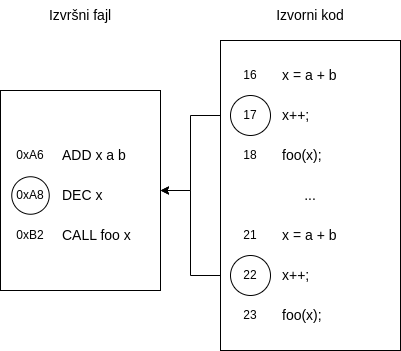
\includegraphics[width=0.6\textwidth]{assets/outlining_breakpoint.png}
  \caption{Vizuelni prikaz odnosa izdvojenog koda u izvornom kodu i izvršnom fajl}
  \label{fig:outlined_breakpoint}
\end{figure}
Ukoliko korisnik postavi tačku prekida na red 17, do prekida će doći i prilikom izvršavanja linije 22 i obrnuto.
Korisnik ne treba da bude svestan postojanja izdvojene funkcije jer on debaguje samo na osnovu izvornog koda.
Za njega, očekivani ishod treba da bude da se program zautavlja samo na redu koji je on izabrao.

% Breakpoint postavlja BreakpointResolver
% BreakpointLocation prosiren da sadrzi opcionu lokaciju u izvornom kodu
% Breakpoint se svakako postavlja na adresu ali ukoliko se lokacija ne poklapa, izvrsavanje se nastavlja dalje. Funkcija \verb|ShouldStop|
% Za postavljanje lokacije se koristi mapiranje lokacje na adresu (outline line table iz CompilaUnit-a)
% A za proveru da li je lokacija dobra se koristi mapiranje adresa+context->lokacija i proverava se da li se lokacije poklapaju
% Postoji i uslov koji moze da se podesi nad celim breakpoint-om ali on se ne proverava u odgovarajuce vreme. Istraziti detaljnije
Rešenje problema nije moguće realizovati u vreme postavljanja tačke prekida, već se provera ispravnosti lokacije radi nakon izazivanja prekida ali pre povratka kontrole korisniku.
Dok klasa \verb|Breakpoint| poseduje sve podatke o grupi tačaka prekida koje su nastale istom komandom, informacije o svakoj pojedinačnoj instanci se nalaze u okviru klase \verb|BreakpointLocation|.
Ona je dopunjena poljem koje predstavlja opcionu lokaciju u izvornom kodu koja odgovara toj adresi i poljem logičkog tipa koje obeležava da li je instrukcija izdvojena.
% Lokacija u izvornom kodu je neophodna samo za podršku izdvojenih instrukcija.
Oba dodata polja dobijaju vrednost prilikom kreiranja tačke prekida na osnovu podataka iz tabela linija.
Dolaskom na tačku prekida u toku izvršavanja radi se provera da li treba vratiti kontrolu korisniku kroz funkciju \verb|ShouldStop| klase \verb|BreakpointLocation|.
U ovom trenutku je potrebno proveriti da li se lokacija sačuvana u polju poklapa sa lokacijom koja odgovara trenutnom stanju procesa.
Način dobijanja trenutne lokacije je isti kao i u prethodna dva poglavlja, uz pomoć trenutne adrese i konteksta.
Ukoliko se lokacije poklapaju, proces će se zaustaviti, a u suprotnom će se prekid ignorisati.
% Nigde u implementaciji ne postoji zavisnost na konkretan način postavljanja tačaka prekida tako da bi isti mehanizam trebalo da funkcioniše 
Posebna pažnja je data da se ova provera radi pre bilo koje druge operacije koja može da izmeni stanje tačke prekida.
Na primer pre uvećavanja brojača aktivacije tačke prekida koji korisnik može da korsiti za napredno debagovanje.

\chapter{Rezultati}
\label{sec:results}

Modifikovanu verziju kompajlera i debagera je potrebno detaljno testirati u različitim mogućim situacijama kako bi se postarali da se prvenstveno ne smanjuje funkcionalnost u odnosu na nemodifikovanu verziju, a zatim i da se zapravo unapređuje debagovanje izdvojenog koda.
Kako je velika količina koda izmenjena, velike su šanse da je došlo do propusta u implementaciji koji nisu detektovani testiranjem na jednostavnim primerima u toku prvobitnog pisanja koda.
To će biti provereno korišćenjem testova.

% LLVM jedinicni i integracioni testovi
% TODO cite
Projekat LLVM već uključuje veliki broj regresionih testova koji pokrivaju skoro svaku podržanu funkcionalnost.
Ti testovi se pokreću koristeći pomoćni alat \verb|lit| (skraćeno za {\em LLVM Integrated Tester}) i sastoje se od fajlova koji sadrže k\^od koji se testira i ugrađene direktive u vidu komantara.
% Direktive mogu da budu ili komande koje se pokreću za izvršavanje testa ili direktive koje zadaju tvrdnje koje test proverava.
Svaki test sadrži bar jednu direktivu za izvršavanje komande. Ona je označena niskom \verb|RUN:| posle koje sledi komanda koja će biti izvršena.
Ta komanda određuje rezultat testa. Ukoliko se ona izvrši uspešno (sa rezultatom 0) onda je test uspešan, u suprotnom je neuspešan.
Komanda se uglavnom sastoji od pokretanja nekog od alata infrastrukture LLVM čiji rezultat se prenosi u alat \verb|FileCheck| koji omogućuava proveru u odnosu na očekivane vrednosti koje su zapisane pomoću \verb|CHECK| direktiva u test fajlu. 
Ukoliko se za kompilaciju projekta LLVM koristio alat \verb|Ninja|, pokretanje regresionih testova se radi komandom \verb|ninja check-llvm|.

% Testovi
Pokrenuti su svi testovi uključeni u LLVM projekat. % Da li se nesto pormenilo prilikom generisanja debug info
Većina testova je uspešno izvršena bez problema. To je bilo i očekivano zato što veliki broj testova i ne radi sa uključenim izdvajanjem koda.
Mali deo testova je neuspešno izvršen zato što proverava specifičan redosled informacija za debagovanje koje su izmenjene modifikovanim kompajlerom.
U tim situacijama, odgovarajući testovi su izmenjeni tako da očekuju pojavljivanje novih etiketa i atributa.
Poslednji, poseban slučaj je činio test koji sadrži istovremeno izdvojen i umetnut k\^od.
Ova situacija nije bila predviđena prilikom pisanja implementacije.
% Umetnut kod zahteva debag lokaciju.
Dotični test se prevremeno zaustavljao zbog neispunjene tvrdnje da poziv funkcije koja može da bude umetnuta unutar funkcije sa informacijama za debagovanje mora da ima lokaciju.
Za taj slučaj je dodata posebna podrška.
Pozivima koji ispunjavaju opisani uslov je postavljena veštačka debag lokacija.
% Kada je provereno da implementacija ne dovodi do regresija
Posle ispravke poslednjeg testa nije uočeno više problema i svi testovi su se uspešno izršavali.

% Primer debagovanja C primera
Sledeće je potrebno isprobati da li implementacija uspešno rešava probleme koje je namenjena da reši.
Demonstracija će biti prikazana na istom primeru koji je predstavljen ranije u listingu \ref{lst:outline_program_example}.
Ponašanje debagera na izdvojenom kodu pre modifikacija je opisano u glavi \ref{sec:izdvajanje_koda_debag}.

% Komande za kompilaciju su iste kao ranije
Kompilacijom sa modifikovanim kompajlerom i proverom informacija za debagovanje izvršnog fajla se može se primetiti da su nove etikete generisane na mestima poziva funkcija i da se adrese poklapaju sa adresama instrukcija u izdvojenoj funkciji.
Pokretanjem debagera na generisanom fajlu i koračanjem po programu dobija se ispis prikazan u slici \ref{lst:outlining_debug_step_after}.
Ukoliko se ovaj ispis uporedi sa ispisom pre modifikacija primećuje se da se program zaustavlja na 3 od 4 izdvojene instrukcije što prethodno nije bio slučaj,
% TODO: dakle radi kod za koracanje i ispisivanje lokcija
Takođe, svaki put kad se zastane ispisuje se poruka koja govori da se proces nalazi u izdvojenoj funkciji.
% c1--; u prethodnom primeru je optimizovano zbog cega je izgubilo lokaciju
Četvrta naredba, \verb|c1--;|, ne izaziva prekid izvršavanja programa.
Istraživanjem je otkriveno da se odgovarajuća instrukcija koja je u početku bila instrukcija sabiranja sa -1, u toku izbora instrukcija zamenila sa instrukcijom dekrementiranja za 1.
Zbog te zamene izgubljen je \verb|outline_id| koji je ta instrukcija originalno imala, stoga nije bilo moguće pronaći adresu te instrukcije prilikom emitovanja asemblerskog koda.
% 
Dakle, još uvek postoji prostor za poboljšanje implementacije.

\begin{figure}[!ht]
\begin{minted}[breaklines, fontsize=\small]{text}
  $ lldb outline
  (lldb) breakpoint set --line 11
  (lldb) run
      9           int y = 1;
      10          
   -> 11          int c1 = x + y;
      12          c1--;
      13          global += 2;
  (lldb) next
      9           int y = 1;
      10          
   -> 11          int c1 = x + y;
      12          c1--;
      13          global += 2;
  Note: this function is outlined.
  (lldb) next
      11          int c1 = x + y;
      12          c1--;
   -> 13          global += 2;
      14          foo(c1, global);
      15          
  Note: this function is outlined.
  (lldb) next
      12          c1--;
      13          global += 2;
   -> 14          foo(c1, global);
      15          
      16          int c2 = x + y;
  Note: this function is outlined.
\end{minted}
\caption{Koračanje po izdvojenom kodu sa izmenjenim debagerom}
\label{lst:outlining_debug_step_after}
\end{figure}

Još jedna implementirana funkcionalnost koju treba proveriti je postavljanje tacaka prekida.
U prethodnom primeru je izgledalo kao da se uspesno postavila tacka prekida na liniji 11 koja je izdvojena.
Ono sto se zapravo desilo je da se tacka postavila na instrukciju poziva izdvojene funkcije koja je dobila lokaciju prve izdvojene instrukcije.
Tek sledecim korakom se zapravo doslo do izdvojene instrukcije.
Umesto te naredbe na redu 11, tacka ce biti postavljena na red 13 kako bi se izbegla prethodna situacija.
Ispis debagera je prikazan na slici \ref{lst:outlining_debug_breakpoint_after}.
Komanda za postavljanje tacke prekida je uspesno odredila adresu koja odgovara zadatoj liniji i pokretanjem programa, proces je zaustavljen na toja adresi.

\begin{figure}[!ht]
\begin{minted}[breaklines, fontsize=\small]{text}
  $ lldb outline
  (lldb) breakpoint set --line 13
  Breakpoint 1: where = outline`outlined_ir_func_0 + 11 at outline.c, address = 0x00005555555551a0
  (lldb) run
      10          
      11  	       int c1 = x + y;
      12  	       c1--;
   -> 13  	       global += 2;
      14  	       foo(c1, global);
      15          
      16          int c2 = x + y;
  Note: this function is outlined.
\end{minted}
\caption{Postavljanje tačke prekida na izdvojenu naredbu sa izmenjenim debagerom}
\label{lst:outlining_debug_breakpoint_after}
\end{figure}

% Dodati novi testovi
Novi regresioni testovi su dodati za kompajler i debager po ugledu na prethodni primer.
Kompajleru se testira uspešno generisanje informacija za debagovanje u svakom koraku kompilacije.
% TODO: debager testovi pokrecu unapred zadate komande i ocekuju odgovarajuci ispis u svakom koraku.
Debager se testira pokretanjem nad programom sa izdvojenim kodom i automatskim zadavanjem komandi koje proveraju ispravnost lokacije, da li se program zaustvio na očekivanim mestima i da li je uspešno postavljena tačka prekida.


% ------------------------------------------------------------------------------
\chapter{Zaključak}
\label{sec:conclusion}
% ------------------------------------------------------------------------------

U okviru ovog rada su opisani proces kompilacije sa akcentom na optimizacijama koda i postupak otklanjanja grešaka u softveru pomoću debagera.
% U okviru ovog rada je opisan proces kompilacije sa akcentom na optimizacijama koda.
% Zatim je opisan postupak otklanjanja grešaka u softveru pomoću specijalizovanih alata, debagera.
Detaljno je objašnjena uloga informacija za debagovanje i problem održavanja tih informacija prilikom izvršavanja kompajlerskih optimizacija.
Za potrebe kompilacije i debagovanja korišćeni su alati infrastrukture LLVM, konkretno kompajler LLVM i debager LLDB.
% Optimizacija izdvajanja koda
% Opisana je optimizacija izdvajanja koda koja pronalazi ponovljene delove koda i izdvaja ih u funkciju kako bi se uštedele memorija programa.
Glavni predmet rada je optimizacija izdvajanja koda koja štedi memoriju programa tako što pomera ponovljene delove koda u zasebnu funkciju i uklanja duplikate.
To smanjenje krajnjeg koda predstavlja problem očuvanju informacija za debagovanje i dovodi do problema prilikom upotrebe debagera.
% Projekat LLVM

% Glavni doprinos
Doprinos ove teze je poboljšanje očuvanja informacija za debagovanje prilikom optimizacije izdvajanja koda u okviru kompajlera LLVM.
One su sačuvane prilikom primene optimizacije, prenete kroz sve faze kompilacije i upisane u sekciju za debagovanje izvršnog fajla.
Na osnovu toga poboljšan je i debager LLDB da iskoristi te informacije kako bi se ostvarilo bolje iskustvo debagovanja.
Dodata je podrška za ispisivanje ispravnih lokacija iz izvornog koda, koračanje i postavljanje tačaka prekida na izdvojenom kodu.
% Za implementaciju je koriščena infrastruktura LLVM, ali se ideja rešenja može preneti i na druge kompajlere i debagere.

% Buduci rad:
% Podrska za MachineOutliner
% Bolja podrska za SelectionDAG
% Podrska za druge ISel implementacije
% Backtrace ne treba da prikaze stek okvire izdvojenih funkcija

Postoji nekoliko pravaca daljeg razvoja.
Predloženo rešenje je moguće implementirati u drugim kompajlerima i debagerima kao što su \textit{GCC} i \textit{GDB}.
Što više alata podržava ovo rešenje, veći broj korisnika će uživati u pogodnostima koje ono pruža.
% Predloženo rešenje je moguće implementirati i u drugim kompajlerima i debagerima.
% Nažalost kompajler GCC trenutno ne podržava optimizaciju izdvajanja koda pa ovo rešenje nije primenjivo na njega, ali se u debager GDB može dodati podrška za proširenje formata DWARF što bi poboljšalo iskustvo prilikom debagovanja programa prevedenog kompajlerom LLVM.
% U okviru same infrastrukture LLVM, moguća su poboljšanja implemenatcije.
Pored toga, moguća su poboljšanja ove implementacije u okviru infrastrukture LLVM.
Trenutno postoji podrška za čuvanje debag lokacija samo iz prolaza \verb|IROutliner|.
Kako se već svakako te informacije spuštaju do mašinski zavisnog međukoda na putu do izvršnog fajla, moguće je dodati podršku i za prolaz \verb|MachineOutliner|.
Pored toga, trenutna implementacija funkcioniše samo za implementaciju \verb|SelectionDAG| za izbor instrukcija.
Iako je to dovoljno za sada, u budućnosti kada implementacija \verb|GlobalIsel| bude prešla u širu upotrebu biće potrebno podržati i nju.
Na kraju, jedna posledica nastala opisanim izmenama je što pregled stek okvira dok je proces zaustavljen u izdvojenoj funkciji prikazuje stek okvir i te izdvojene funkcije.
Kako ona ne postoji u izvornom kodu, korisniku ne treba da bude prikazana prilikom debagovanja.
Suprotna stvar se dešava kada je proces zaustavljen u umetnutom kodu, gde se konstruiše veštački stek okvir koji ne postoji u toku izvršavanja, ali korisnik očekuje da bude prisutan.
% Što se tiče razvoja van projekta LLVM,
% predloženo rešenje je moguće implementirati i u drugim kompajlerima i debagerima kao što su \textit{GCC} i \textit{GDB}.

% ------------------------------------------------------------------------------
% Literatura
% ------------------------------------------------------------------------------
\literatura

% ==============================================================================
% Završni deo teze i prilozi
\backmatter
% ==============================================================================

% ------------------------------------------------------------------------------
% Biografija kandidata
\begin{biografija}
  \textbf{Vladimir Vuksanović} je rođen 2. januara 1999. godine u Užicu.
  Tamo je završio osnovnu školu i prirodno-matematički smer Užičke gimnazije.
  Posle toga je upisao informatički smer na Matematičkom fakultetu 2017. godine.
  Osnovne studije je završio za 4 godine sa prosekom 9,82.
  Nagrađen je kao jedan od najuspešnijih studenata generacije od strane katedre za računarstvo i informatiku i dobitnik je nagrade "Nedeljko Parezanović".
  Iste godine je upisao master studije na Matematičkom fakultetu takođe na smeru Informatika. 
  Pred kraj studija je radio praksu u kompaniji Sirmija posle čega se tamo zaposlio kao softverski inženjer.
  Tamo radi na programiranju sistemskog softvera, primarno na projektima vezanim za infrastrukturu LLVM.
\end{biografija}
% ------------------------------------------------------------------------------

\end{document}
